\setstretch{1.0}
\chapter{Dynamic recruitment of resting state subnetworks}\label{chap_kmeans}

In Chapter \ref{chapter_cca}, a new approach to measuring the 5-dimensional signature of dynamic functional connectivity in MEG was developed, however it was only tested on a single subject's worth of resting state data. What the results suggested is that multiple spatial modes of connectivity exist within established resting state networks, so here we investigate the nature of these modes across two group studies. Our results show that, when functional connectivity is assessed in small time windows, the canonical sensorimotor network can be decomposed into a number of transiently synchronising sub-networks, recruitment of which depends on current mental state. These rapidly changing sub-networks are spatially focal with, for example, bilateral primary sensory and motor areas resolved into two separate sub-networks. The likely interpretation is that the larger canonical sensorimotor network most often seen in neuroimaging studies reflects only a temporal aggregate of these transient sub-networks. Our approach opens new frontiers to study resting state network (RSN) dynamics, showing that MEG is capable of revealing the spatial, temporal and spectral signature of the human connectome. 

\doublespacing

\section*{Introduction}
Having introduced the methodology to assess amplitude envelope correlations between two clusters of data in Chapter \ref{chapter_cca}, we can now use it to further investigate the dynamical properties of resting state networks (RSNs). Early investigations into RSNs revealed a small handful of robust, large scale functional networks \citep{Biswal1995,Raichle2001,Fox2005,Beckmann2005,Smith2009,Brookes2011}, where their topographies have been derived with stationary methods, meaning that the underlying transient processes which define the network are obfuscated. The pipeline developed in Chapter \ref{chapter_cca} in conjunction with the high temporal resolution of MEG data, means we can probe the behaviour of connections at much shorter time scales than previously attainable (a few seconds rather than minutes, or hours). In the previous chapter, to accommodate the hundreds of connectivity images generated by a sliding window CCA, we used an eigenvalue decomposition to look for specific modes of connectivity. The key finding was that we can decompose a network of interest into smaller sub-networks. However this was conducted in a single subject and in resting state data, so we couldn't comment extensively on the nature of these sub-networks or their functional role. However,  from what we have seen, we can propose a hypothesis about these modes; they are transiently synchronising subnetworks (TSNs), which rapidly form and dissolve based on the current mental task, and their temporal aggregate may resemble the static resting state networks (RSNs).  

In this chapter we investigate these phenomena further by assessing two paradigms of the sensorimotor network in two group studies, the first is a simple motor task embedded into a resting state paradigm and the second is a more complex cognitive task. Instead of eigenvalue decomposition, we use a powerful vector quantisation method called K-means clustering \citep{MacQueen1967} to find repeating patterns of functional connectivity and investigate how these sub-networks are modulated by tasks. Section \ref{sec_kmeans_methods} discusses the experimental procedure and describes the pipeline to fuse CCA with K-means to generate the sub-networks. Section \ref{sec_kmeans_results} shows the results of such an analysis and reveals a series of robust subnetworks that rapidly form and dissolve based on the current mental state.

\section{Methods}\label{sec_kmeans_methods}
\subsection{Data acquisition}

Two separate MEG datasets were acquired. The first was designed as a ‘resting state’ recording with an intermittent self-paced motor response. The second comprised a cognitive task. Diagrams of the paradigms are in Figure \ref{figure_5_0}

\textbf{Dataset 1} -- \textit{Self-paced motor:} Ten volunteers (8 male, 2 female aged 25±4 years (mean ± SD)) were asked to lie supine in the MEG system and execute a button press with the index finger of their non-dominant hand. Subjects were told that button presses should be repeated infrequently (approximately once every 30s) for a total of 1200s, and that they should not count in the period between presses. Ten right handed subjects were recruited. Button presses were recorded using a keypad.

\textbf{Dataset 2} -- \textit{Sternberg working memory task:} Eleven subjects (7 male, 4 female, and aged average 31±6 years (mean ± SD)) were recruited to this study. In the task, a single trial comprised of the presentation of two example visual stimuli (arbitrary black abstract shapes on a grey background, shown for 600 ms with 1s between onsets); this was followed by a 6 s maintenance period and a third probe stimulus which was shown for a duration of 3 s. The subject was asked to respond, via a right handed button press (index finger), if the probe stimulus matched either of the two example stimuli. A single block comprised three trials followed by a rest phase lasting 36 s; 15 blocks were presented to each subject. The probability of a target (i.e. the probe matched one of the two example stimuli) was 0.5.

\begin{figure}[b!]
\begin{center}
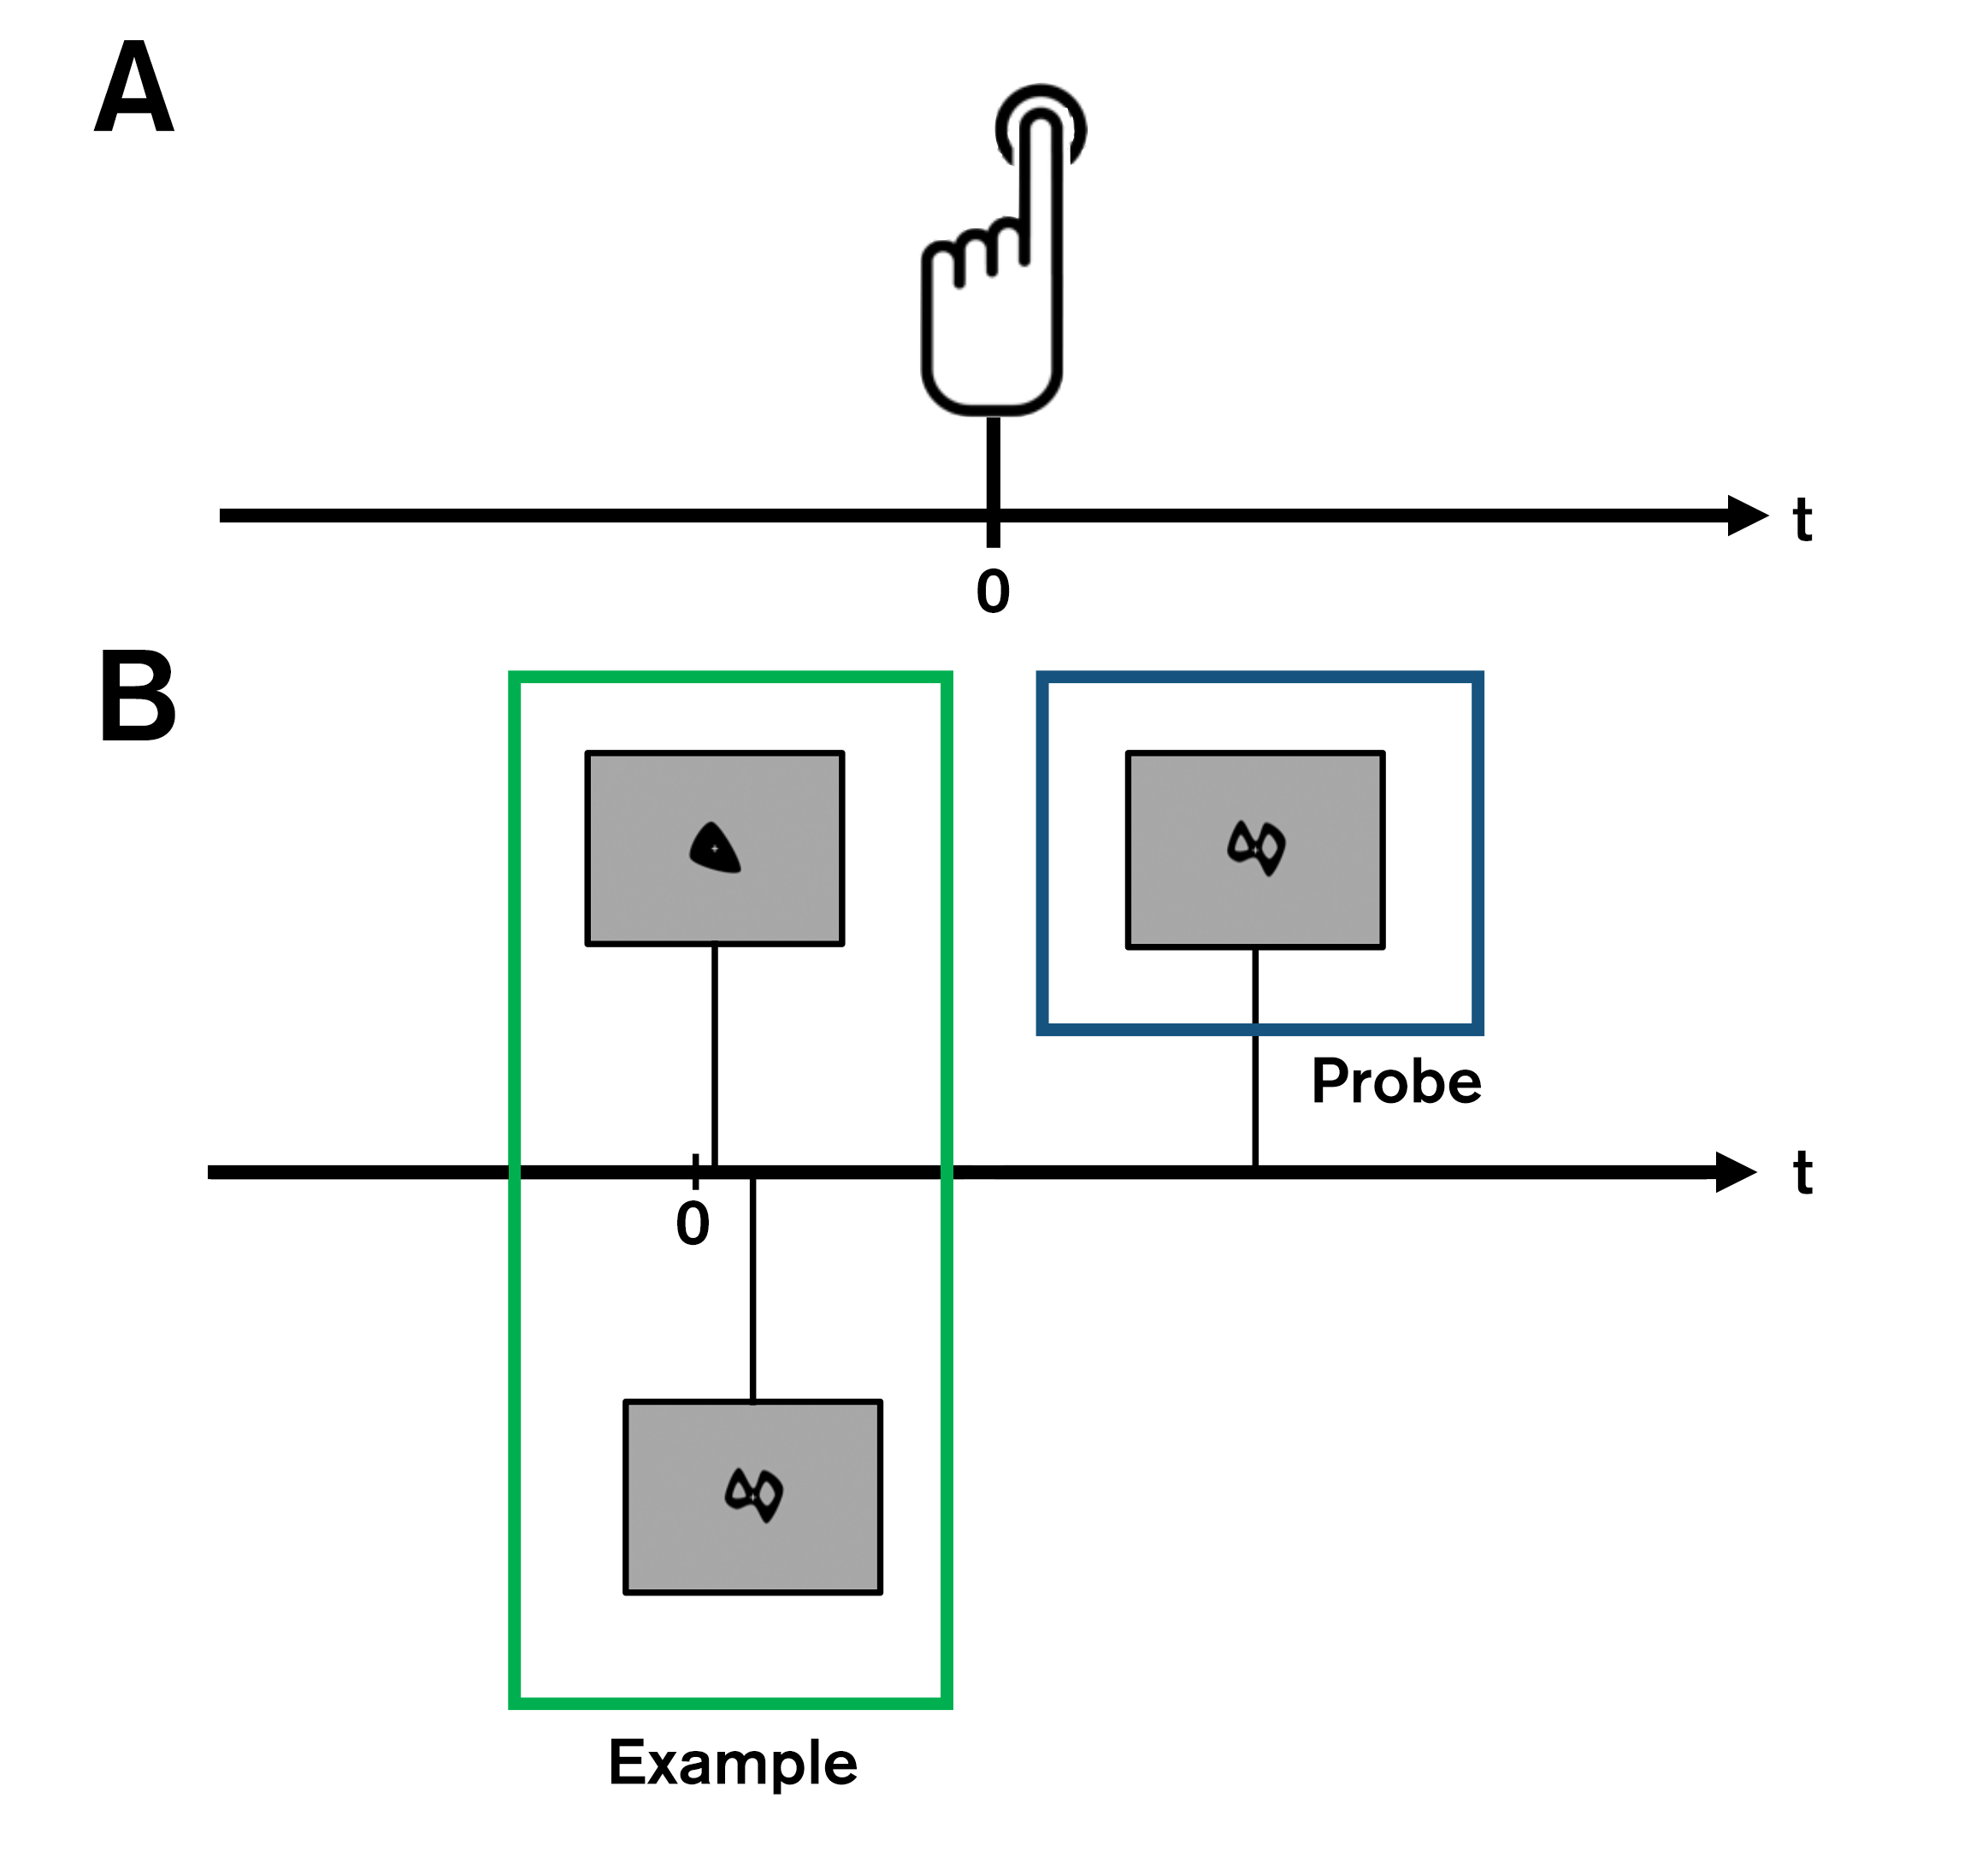
\includegraphics[width=0.8\linewidth]{./images/chapter5/Figure_0.png}\caption{Diagrams of the experiments conducted. A) The self paced motor task. B) The Sternberg working memory task.}\label{figure_5_0}
\end{center}
\end{figure}

These two paradigms both contain a motor response (a button press). However, the difference between them allows contrast between simple motor action, infrequently performed during the resting state, and similar motor action set within a complex cognitive paradigm. It was reasoned that if TSN signatures were integral to sensorimotor processing, then equivalent TSNs should be observed for both tasks. In addition, the Sternberg task would allow investigation of TSN dynamics for fast and slow reaction times. Both experiments were approved by the University Of Nottingham School Of Medicine Ethical Committee. 

All MEG data were collected using the CTF MEG system in Nottingham, acquisition procedures followed are the same as those laid out in Chapter \ref{sec_data_acq}, with the only exception being that the self paced motor data, which was acquired at a sampling rate of 1200 Hz. 

\subsection{Data analysis}

A data processing pipeline which builds upon that in Chapter \ref{chapter_cca} was developed to image the hypothesised TSNs. This is shown schematically in Figure \ref{figure_5_1}. Again, functional connectivity was estimated as the correlation between the amplitude envelopes of band limited neural oscillations in left and right regions of the static sensorimotor network. Since previous studies show that sensorimotor network connectivity is strongest in the beta band (see results in Figure \ref{fig_4_7} as well as studies by  \citealp{Brookes2011a,Hipp2012,Brookes2014}) analyses were limited to 13-30Hz. Our technique used: 1) a spatial filter to project sensor space MEG data into brain space and dynamic multivariate leakage reduction to ameliorate the confounds of source space signal leakage. 2) A sliding window canonical correlation analysis (CCA) was used to estimate the spatial signature of transient functional connectivity within each time window. 3) Vector quantisation (k-means clustering) to cluster connectivity images into repeating spatial patterns; it is these patterns which form transiently synchronising sub-networks (TSNs). These steps are each described further below.

\subsubsection{Source localisation and leakage correction}
Source localisation was carried out using an adaptive beamformer \citep{VanVeen1997,Robinson1999}. Covariance was computed in the beta band using a time window spanning the whole experiment \citep{Brookes2008}. Regularisation was applied to the data covariance matrix using the Tikhonov method, with a regularisation parameter set to ensure a condition number of 100. The forward model was based upon a dipole approximation \citep{Sarvas1987} and a multiple local sphere head model \citep{Huang1999}. Dipole orientation was determined using the scalar method discussed in Chapter \ref{sec_334}. Source timecourses were computed at the vertices of a regular (8 mm) grid spanning the volume enclosed by the static sensorimotor network. The network mask was based upon an atlas derived using spatial independent component analysis applied to fMRI data \citep{Filippini2009}. The seed cluster was placed in the right hemisphere and the test cluster in the left hemisphere. Beamformer estimated timecourses for all voxels within the mask were divided by hemisphere; a ‘seed’ cluster was defined, containing all voxels in the left hemisphere enclosed by the mask; likewise a ‘test’ cluster was defined containing all voxels in the right hemisphere enclosed by the mask (see Figure \ref{figure_5_1}). 

Leakage correction was performed using the multivariate orthogonalisation method introduced in Chapter \ref{chapter_cca}. However, here we note that the implicit assumptions of non-stationarity in functional connectivity brings with them implications for such standard methods to mitigate the effects of leakage. In Chapter \ref{chapter_cca}, we assumed stationarity, and performed a single leakage correction step for the whole dataset, whereas it has been proposed  by \cite{Hipp2012} that a dynamic approach is required, correcting small time-windows individually. The advantage of the former is that the leakage correction will be more precise as it is based on more data. The advantage of the latter is that it will be robust for non-stationary data. In fact it can be shown (see Appendix \ref{sec_dyn_leak}) that when measuring functional connectivity across multiple time windows, if changes in variance in either a seed or test cluster timecourse are expected between windows, then dynamic leakage reduction is essential to ensure unbiased functional connectivity estimation. For this reason, in the present work, we used a dynamic multivariate regression approach to eliminate signal leakage between the seed and test clusters on a window-by-window basis.

\subsubsection{Transient functional connectivity via CCA}
Following source localisation and leakage reduction, beamformer projected data for all voxels in the seed and test clusters were Hilbert transformed and their associated analytic signal computed. The absolute value of the analytic signal was then derived, generating timecourses of the envelope of beta oscillations for every voxel. These envelope timecourses were down-sampled temporally to 50 Hz to improve computational efficiency. We again used Canonical Correlation Analaysis (CCA; Chapter \ref{chapter_cca}) to asses functional connectivity. In the present context, CCA was applied across voxel timecourses to assess relationships between the beta envelopes in the seed and test clusters. A sliding window framework was used with canonical correlation measured independently within either 6 s windows (self-paced Study) or 3 s windows (Sternberg study). (The difference in window width across the two studies was to account for the shorter trial duration in the Sternberg task.) Note that the window lengths are considerably shorter than those in Chapter \ref{chapter_cca}, where windows were 30 s. The narrowing of the the windows allow us to probe changes in functional connectivty on temporal scales unavailable in the previous chapter. Sliding the window in time (using either 1 s steps (self-paced Study) or 0.25 s steps (Sternberg study)) facilitates generation of many images, each showing the transient spatial signature of functional connectivity. These images were transformed spatially into MNI space using FMRIB Linear  Image Registration Tool (FLIRT) in FSL \citep{Jenkinson2012}. Images were then concatenated across all 10 subjects for the self-paced study, and all 11 subjects for the Sternberg study.

In addition to the sliding window images, static images were also derived using the same CCA method, but with one single window spanning the entire duration of the experiment. These static images highlight voxels that contribute maximally to correlation between the seed and test clusters, over all time. They were transformed spatially into MNI space using FLIRT, averaged across subjects and used for direct comparison with the TSNs derived from the shorter sliding windows.

\subsubsection{K-means Clustering}
Using the sliding window CCA approach, within a multi-subject dataset, several thousand images of connectivity are generated. (Specifically 11,940 and 25,272 for the self-paced and Sternberg studies respectively). This means that an automated process of grouping and classifying these images is desirable. K-means clustering \citep{MacQueen1967} is method of vector quantisation which has been used in recent fMRI experiments \citep{Allen2014,Liu2013} to detect repeating patters of connectivity. This is distinct to the principal component analysis approach used in Chapter \ref{chapter_cca}, as data is clustered into groups based in its euclidean geometry in \textit{f}-dimensional space, rather than decomposed from data reduction methods. Secondly K-means doesn't require the results to be orthogonal, allowing for overlap in network topographies of which PCA  necessarily avoids. If we assume a total of $n_o$ sliding windows across the experiment, then K-means partitions those $n_o$ connectivity images into $k$ states. To do this, we first note that the images exist in an $f$ dimensional space (where $f$ represents the total number of voxels in the seed and test cluster combined). $k$ points are then inserted into this space to form the centre of derived clusters and the K-means algorithm looks to minimise the within cluster sum of squares of Euclidian distance to the mean, over multiple iterations. Mathematically: 

\begin{equation}
\underset{\mathbf{S}}{\text{min}} \sum_{j=1}^{k} \sum_{\mathbf{I}_i \in \mathbf{S}_j}\parallel\mathbf{I}_i - \mathbf{\mu}_j\parallel^2 \label{eqn_5_1}
\end{equation} where $\mathbf{I}_i$ represents the  $i$\textsuperscript{th} connectivity image and $\mathbf{\mu}_j$ is the mean of the points in each projected group, $\mathbf{S}_j$. Physically, these groupings represent images depicting similar functional connectivity patterns which consistently reoccur. We term these repeating patterns transiently synchronising sub-networks (TSNs). Figure \ref{figure_5_00} shows a graphical representation of the K-means. Note that in our investigations we chose $k=8$.


	\begin{figure}[b!]
		\begin{center}
			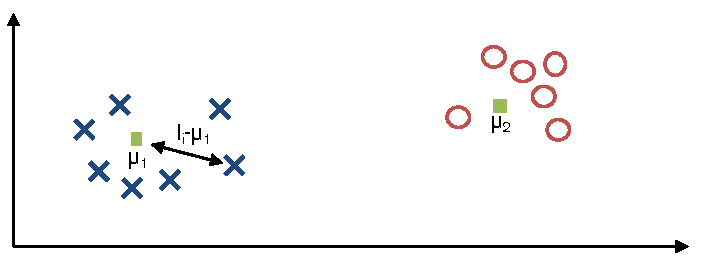
\includegraphics[width=0.9\linewidth]{./images/chapter5/kmeans.pdf}
			\caption{Schematic representation of K-means clustering in 2-dimensional space, with \textit{k}=2. The green squares represent the group's center of mass ($\mu$) and clusters are determined by which group combinations minimise the distance between $\mu$ and the data. \label{figure_5_00}}
		\end{center}
	\end{figure}



\begin{landscape}
	\begin{figure*}
		\begin{center}
			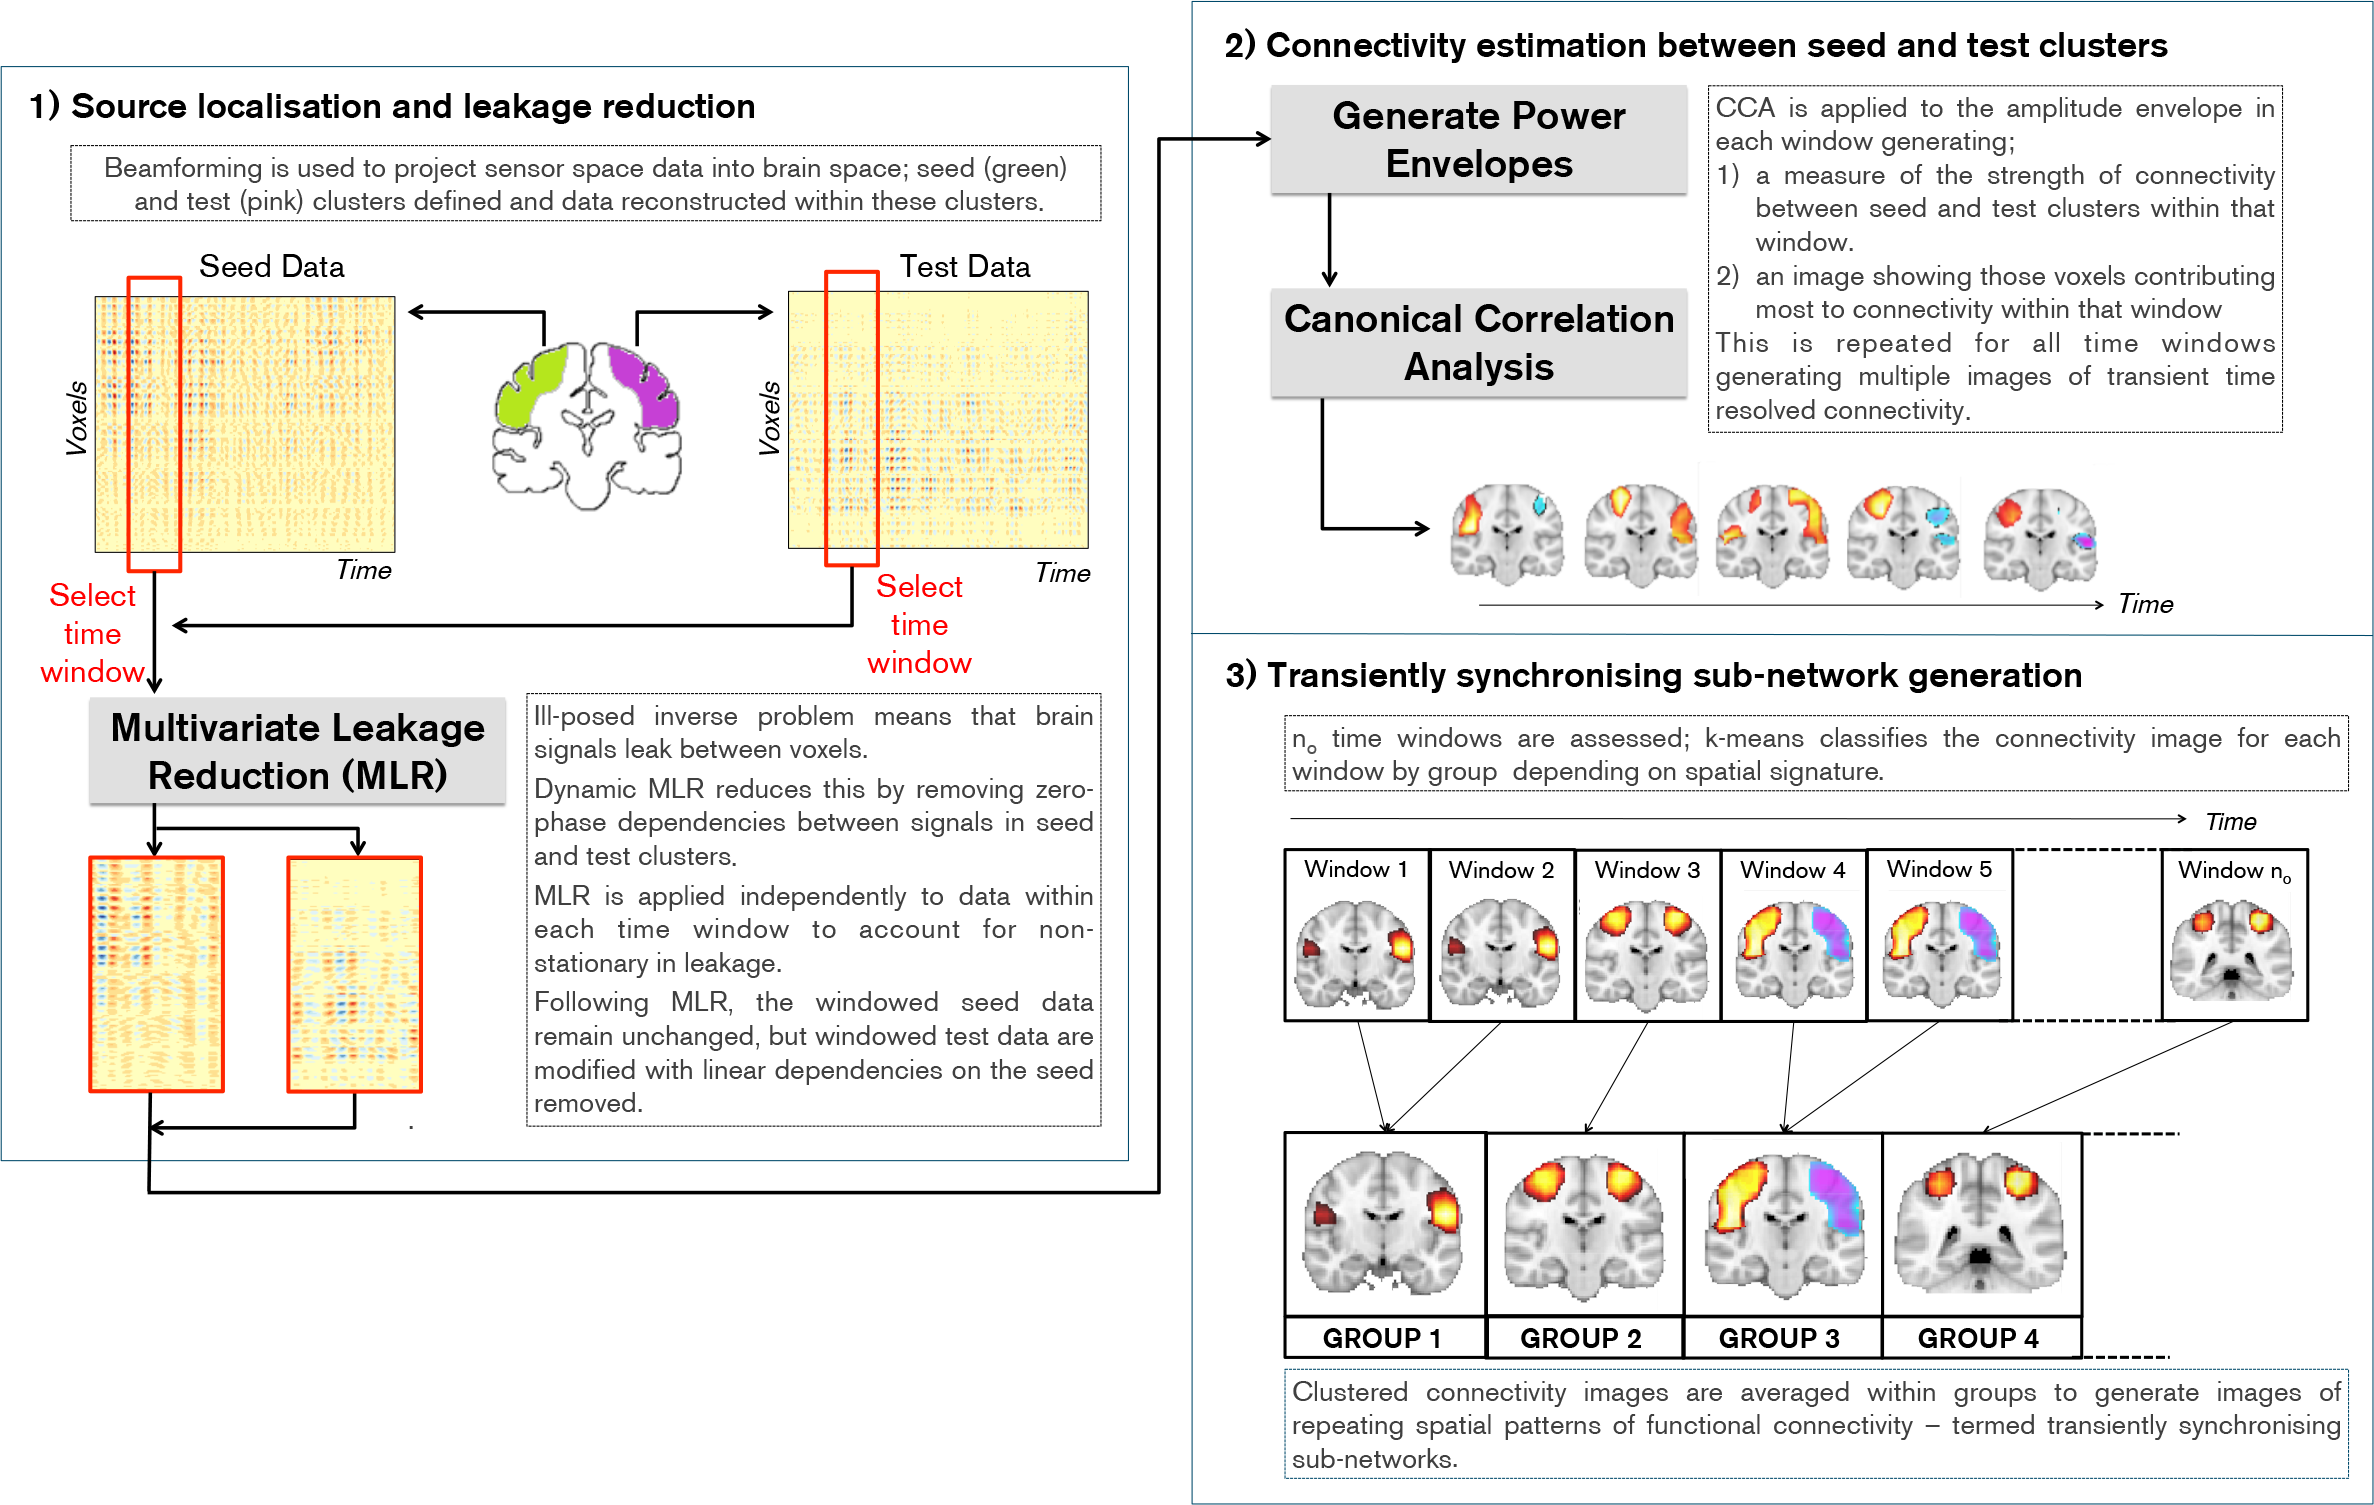
\includegraphics[width=0.9\linewidth]{./images/chapter5/Figure_1.png}
			\caption{Schematic diagram showing the processing pipeline used to extract transiently synchronising networks \label{figure_5_1}}
		\end{center}
	\end{figure*}
\end{landscape}

\subsubsection{Testing TSN robustness}
Our primary hypothesis is that the derived TSNs are spatially distinct (from each other and from the static network) and robust across subjects and datasets. The method outlined above offers a means to capture these spatial patterns. Statistical tests were then sought to validate their robustness. We devised three analyses:

\textbf{1) Miss-a-TSN:}
We first tested whether any of the 8 derived TSNs were redundant (i.e. not required to explain the data). To do this, a single CCA derived connectivity image was selected and its best fitting TSN selected. The percentage of variance in this image, explained by the best fitting (scaled) TSN, was then calculated. This process was repeated for all connectivity images within each subject, and the mean variance explained calculated. This analysis was repeated a further 8 times; on each iteration, a different TSN was removed from the basis set and replaced with the average network (generated as the mean across all connectivity images and subjects). We hypothesised that replacement of any one TSN with the average map would evoke a significant drop in variance explained. Significance was determined using a two-sided signed rank test of the null hypothesis that this difference originated from a distribution whose median is zero. The threshold for significance ($p < 0.05$) was Bonferroni corrected (to \textit{p}\textsubscript{corrected} < 0.0065) to account for multiple comparisons across the 8 TSNs. This test was carried out three times: On the self-paced dataset, on the Sternberg dataset, and finally on just the resting state phase of the self-paced dataset in order to determine whether any of the derived TSNs were only observable during the task.

\textbf{2) Miss-a-subject:}
We next assessed robustness across subjects by testing the hypothesis that TSN maps, derived via k-means, explained the data significantly better than the canonical (static) network map. For this purpose, we first selected a subject and removed their data from the full dataset; k-means was then run on the remaining ($N – 1$) subjects to derive a TSN basis set. A “sham” TSN basis set was also derived in which, rather than each connectivity image being assigned to a group via Equation \ref{eqn_5_1}, it was assigned randomly. Note that these “sham” maps are computed without considering temporal structure in the measured connectivity (i.e. assuming stationarity), and for this reason we term them “static pseudo-networks”. This process generated two basis sets, both using $N – 1$ subjects. These two basis sets were then used to explain the variance in the remaining subject. We reasoned that if the TSN maps were robust across subjects then they would explain significantly more variance in the missing subjects’ data than static pseudo-networks. This analysis was repeated for all subjects, generating a set of values of variance explained. We then tested whether TSN maps explained more variance than static pseudo-networks across $N$ iterations of the missing subject.

\textbf{3) Cross-dataset validation:}
The above tests were run within datasets (i.e. either using Sternberg data only, or self-paced data only). However, if the TSNs derived using k-means are genuine transient networks that support sensorimotor function, then they should generalise to any task (or indeed the resting state). A cross-dataset validation was therefore performed in which we used the TSN basis set from the self-paced experiment to explain the Sternberg data, and vice versa. The TSN basis set from the self-paced data was taken along with an equivalent set of 8 static pseudo-networks. We reasoned that if the TSN maps were not robust, the TSN basis set from the self-paced study would explain no more variance in the Sternberg data than the static pseudo-networks. A null distribution was formed via generation of 2000 separate basis sets based upon different realisations of the static pseudo-networks, and we tested our hypothesis that the genuine TSN set (from the self-paced data) would explain significantly more variance in the Sternberg data than the sham basis-sets. This analysis was then reversed, and the Sternberg basis set used to explain the self-paced data, employing an identical methodology.

\subsubsection{Task induced change in transiently synchronising sub-networks}
Our secondary hypothesis was that, on task initiation, efficient neural processing would favour recruitment of a specific set of sub-networks. To measure how a task affected the likelihood of occurrence of a network, for each TSN, we first constructed a binary timecourse. This was computed across all task trials and subjects and was based on k-means grouping; it contained a 1 if the current window belonged to the TSN group of interest, or a 0 otherwise. This vector was summed across task trials (over all subjects) and divided by the total number of trials; the result is a timecourse showing the probability of a specific TSN being selected for any time window within a trial (see Figure \ref{figure_5_2}). Dividing these timecourses by the overall fraction of windows classified in the group enabled measurement of the fractional change in probability of observing any one network, at any time point within a trial. A deflection in these timecourses would highlight that the TSN in question was more, or less likely to be observed within that time window.

	\begin{figure*}[h]
		\begin{center}
			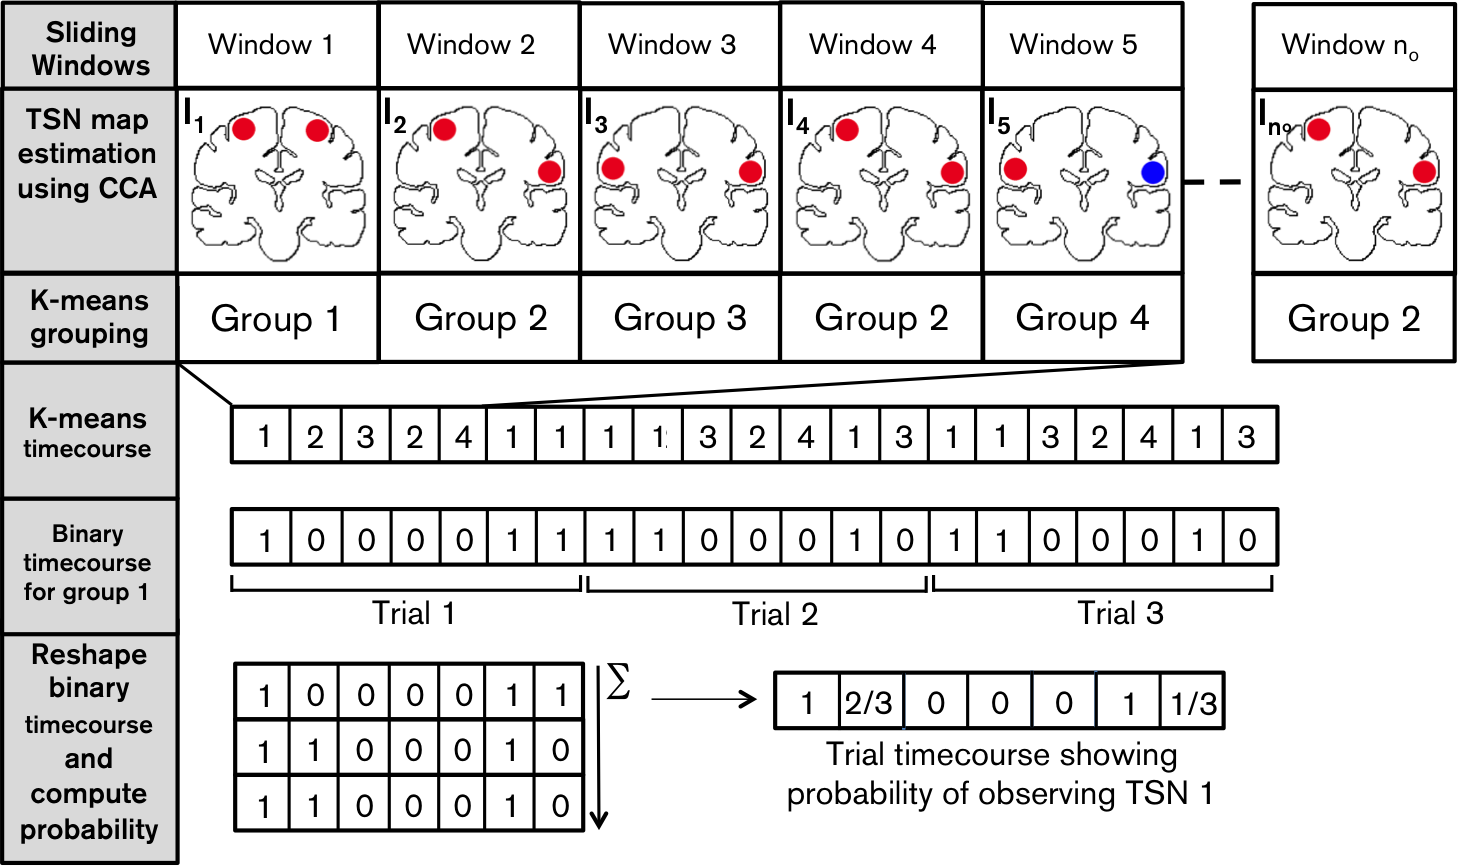
\includegraphics[width=\linewidth]{./images/chapter5/Figure_2.png}
			\caption{Schematic diagram showing the processing pipeline used to extract transiently synchronising networks \label{figure_5_2}}
		\end{center}
	\end{figure*}

Finally, a method was devised to confirm that any observed deflection in the probability timecourses was due to localised changes in functional connectivity within the TSN in question. This was achieved via a ‘point-to-point’ transient connectivity analysis. To compute point-to-point connectivity, firstly, two points (a seed and test) were selected based upon the peaks in a TSN map; source timecourses were then estimated using the beamformer. A sliding window was allowed to shift across the timecourses and a dynamic (univariate) leakage reduction applied within each window. Following leakage reduction, the amplitude envelope of both the seed and test timecourses (within each window) was computed via Hilbert transformation and connectivity estimated, via (univariate) correlation, within each window. These connectivity timecourses were averaged across task trials within each individual subject. To allow for changes in the temporal scale of functional connectivity, this process was repeated for window widths ranging from 2 s to 48 s, in the case of the self-paced motor study, and 2 s to 10 s in the case of the Sternberg study. (Note such variation in window widths is impractical for CCA due to computational load.) To determine the statistical significance of task-induced changes in connectivity, the mean variances explained in windows encapsulating the event of interest (the button press) and for windows only capturing rest, were computed and the difference calculated. This was repeated for each subject individually and statistical significance of the difference in measured connectivity between task and non-task windows was computed.

\section{Results}\label{sec_kmeans_results}
\subsection{Transiently synchronous sub-network generation and evaluation}

Figure \ref{figure_5_3} shows TSN maps for the self-paced (A) and Sternberg (B) tasks. Our hypothesis that multiple, spatially distinct and focal TSNs would be observed is supported by Figure \ref{figure_5_3}, which shows that spatial patterns representing transient functional connectivity differ in time. In the Self-paced dataset (Figure \ref{figure_5_3}A), \textbf{TSN1} covers bilateral primary motor and sensory cortex and extends inferior to S2. \textbf{TSN2} only covers primary M1 and S1 regions whilst \textbf{TSN5} captures only bilateral S2. \textbf{TSN6} and \textbf{TSN8} separate anterior and posterior sensorimotor regions: assessment of the peak locations reveals MNI coordinates of (-36,24,60) mm and (40,-22,60) mm for \textbf{TSN6} which equate to the left and right precentral gyri (Brodmann Area 4). MNI coordinates for \textbf{TSN8} were (30,-38,58) mm and (34,-30,60) mm; the peak in right hemisphere is centred on postcentral gyrus (Brodmann area 3) and the peak in left hemisphere is less than 1 voxel from the postcentral gyrus (Brodmann area 3). This evidence shows that bilateral sensory and motor cortices form independent transient networks and our method facilitates their separation. In addition to positive correlations, negative correlations are also observed in \textbf{TSN3}, showing that the method captures windows in which the beta envelopes in the left and right sensorimotor strips are anti-correlated. Finally, \textbf{TSN4} highlights a spatially asymmetric TSN (left M1/S1 and right S2) and \textbf{TSN7} depicts a unilateral response. Results for the Sternberg (Figure \ref{figure_5_3}B) task are similar (Figure \ref{figure_5_3}A) and again include anti-correlated networks (\textbf{TSN2} and \textbf{TSN3}), bilateral S2 (\textbf{TSN5}), and a spatially asymmetric network (\textbf{TSN6}) covering left M1/S1 and right S2. Motor and sensory cortices (\textbf{TSN7} and \textbf{TSN4}) are again separated. In addition to the clear similarity across these two completely independent experiments, note also the highly focal nature of the TSN maps. In particular note that even within the seed cluster (where no leakage reduction is applied) the regions corresponding to the motor and somatosensory have sufficiently different time series to each other for them to be separated by our analysis. Also note that two of the TSNs, namely the bilateral M1 and S2 subnetworks highly resemble the two modes derived from our single subject in Chapter \ref{chapter_cca}.

For comparison, Figures \ref{figure_5_3}C and \ref{figure_5_3}D show static connectivity images generated using the self-paced and Sternberg datasets respectively. These images were generated using the same CCA approach, but with a single time window capturing the entire experiment.  In contrast to the TSN maps, the static map is less spatially specific. Whilst clear foci are observed, they appear to spread across primary sensory and motor regions, and the map extends down to S2 (albeit at a lower threshold).  Most importantly, the subtle spatial dynamics observed in the TSN measurements are missed by the static approach.

\begin{figure*}[h]
	\begin{center}
		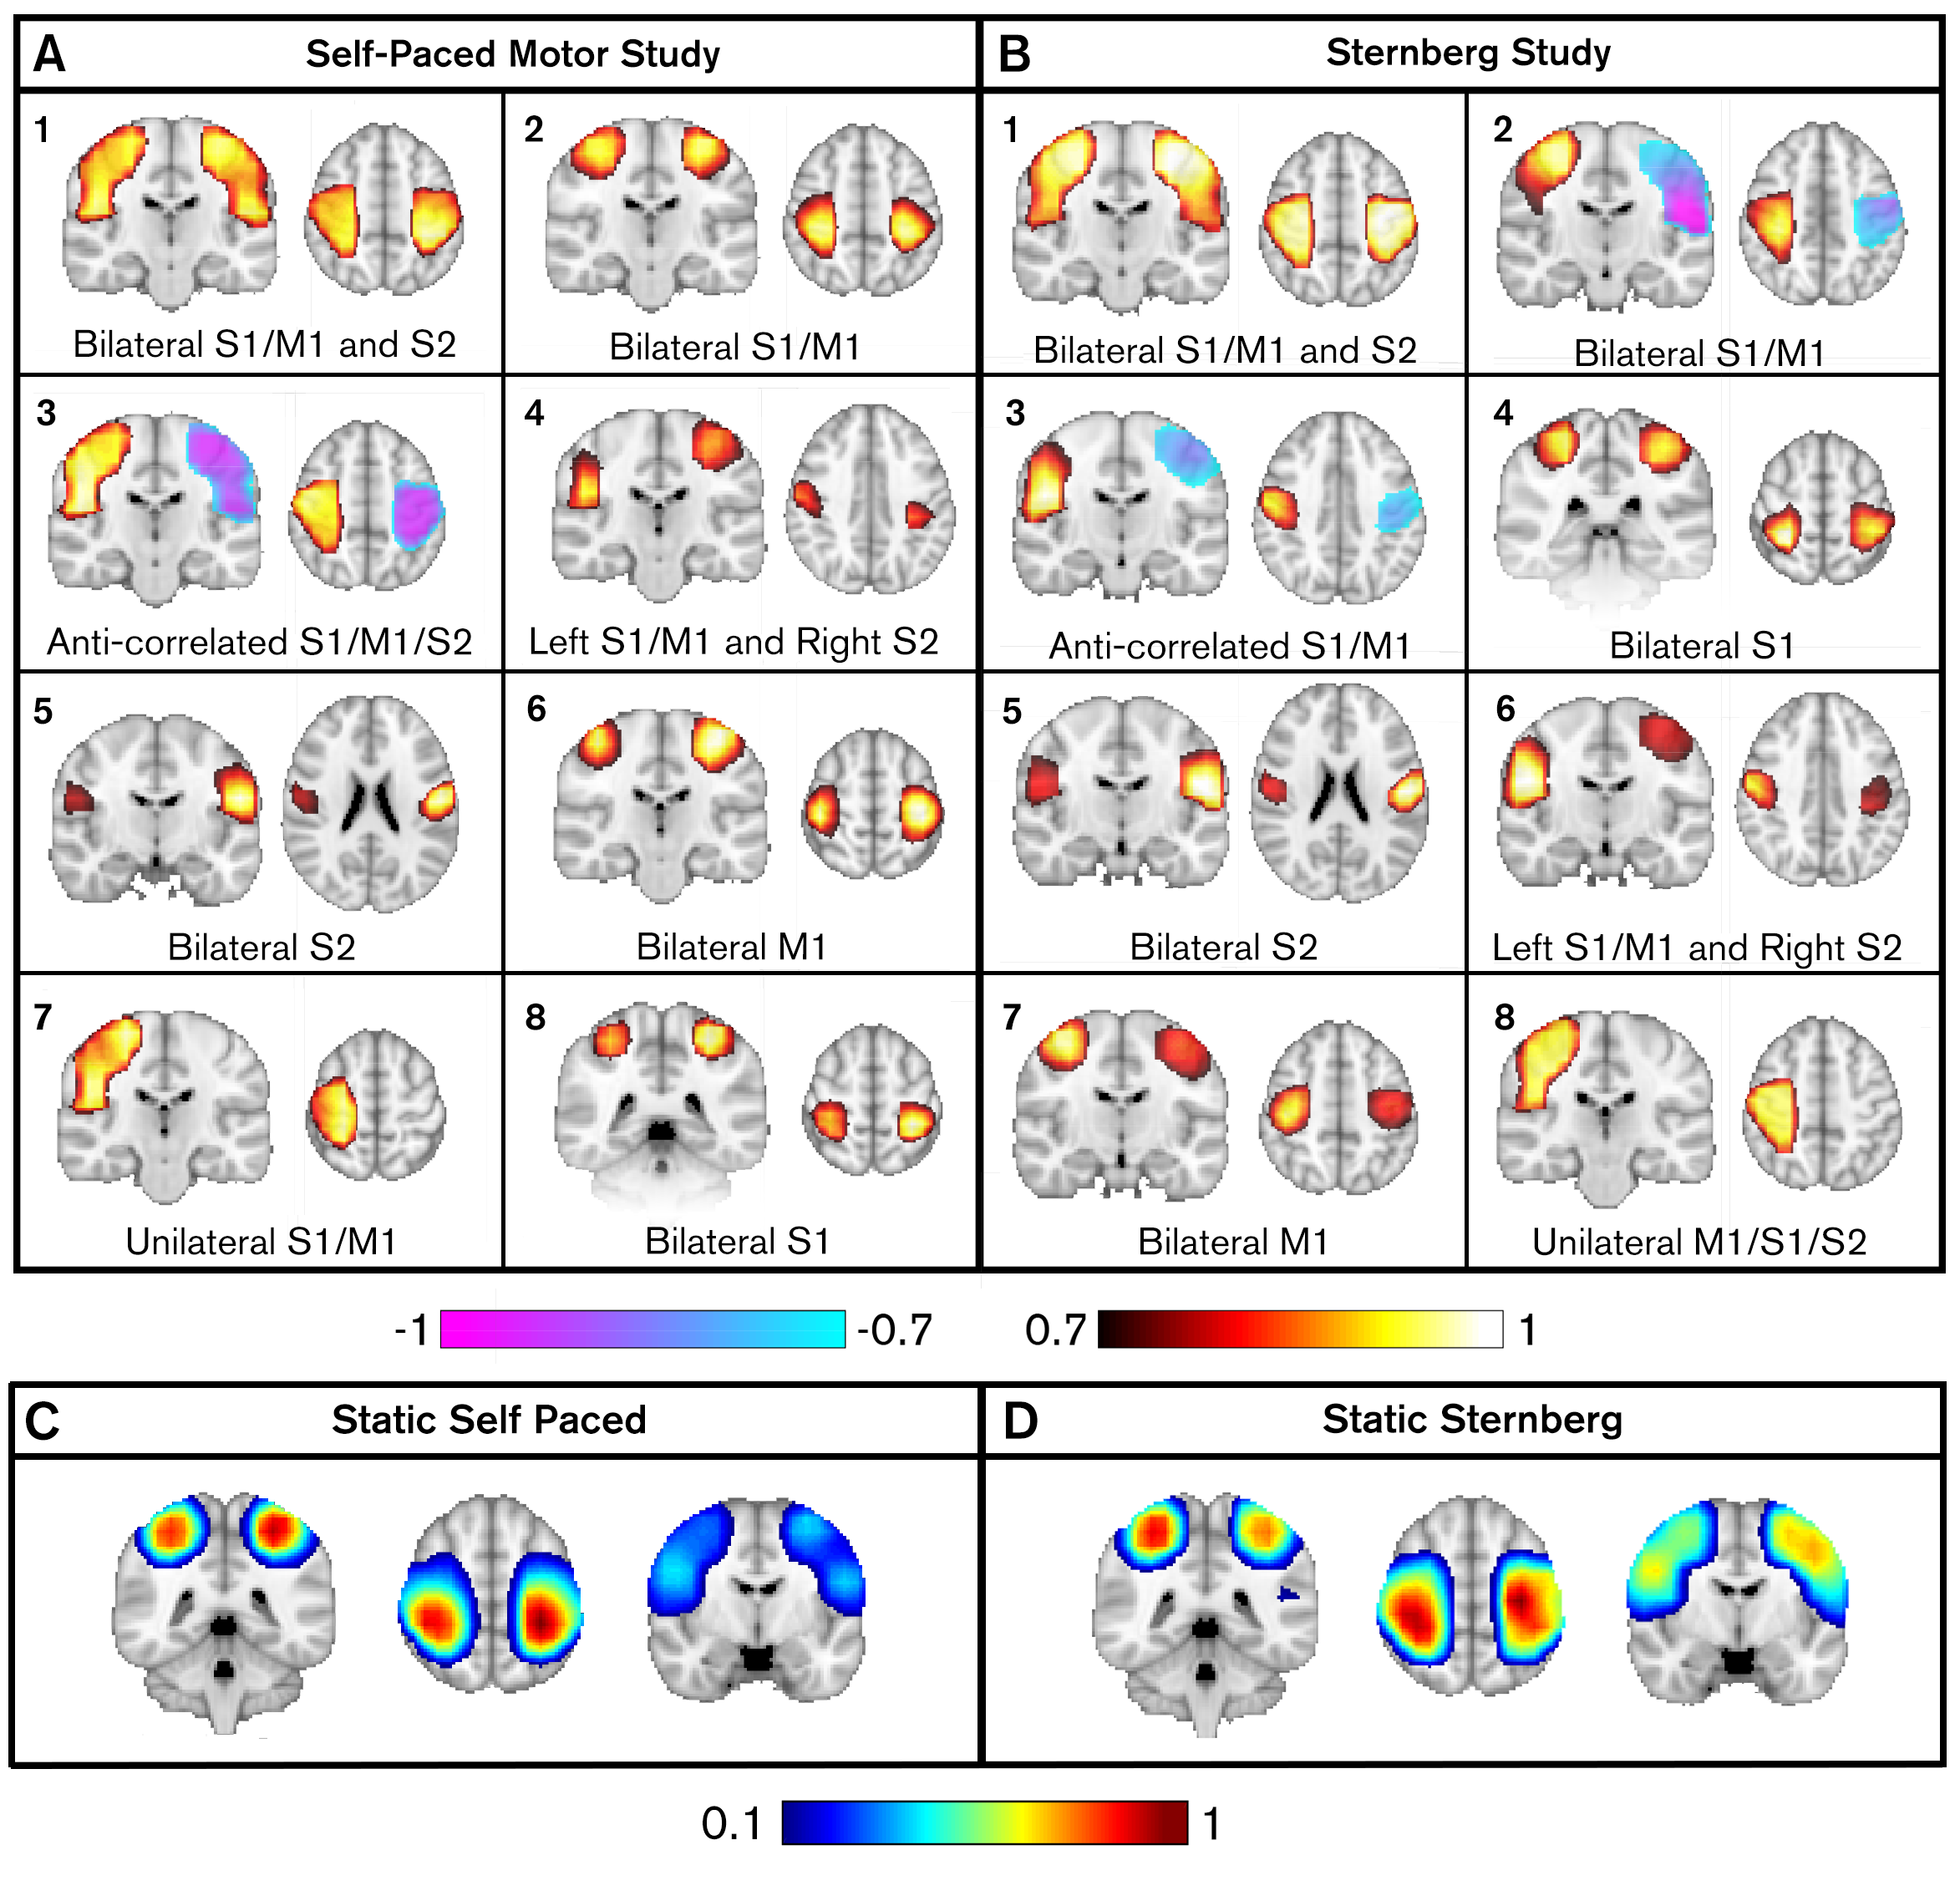
\includegraphics[width=\linewidth]{./images/chapter5/Figure_3.png}
		\caption{Transiently synchronous sensorimotor sub-networks generated using two independent datasets. The left hand side (A) shows a 10-subject dataset in which participants executed an infrequent self-paced button press. The right hand side (B) shows an 11-subject dataset in which participants were involved in a Sternberg working memory task. Note the equivalence of the observed transient connectivity images. Note also the highly focal nature of the spatial topographies. (C-D)  Static connectivity images generated using a window spanning the entire experiment. \label{figure_5_3}}
	\end{center}
\end{figure*}

The robustness of each individual TSN was tested using a “miss-a-TSN” analysis. We tested how much variance in the $n_o$ connectivity images could be explained by our TSN maps, and whether replacing a single TSN with a static network caused a significant drop in the variance explained. The 8 TSNs in Figure \ref{figure_5_3}A explained 71 \pm 3 \% of variance in the self-paced connectivity images. Replacing a single TSN with the static network gave rise to a significant (\textit{p}\textsubscript{corrected} < 0.05) drop in explained variance for 6 of the 8 TSNs. The exceptions were TSN1 (\textit{p}\textsubscript{corrected} = 0.08) and TSN7 (no trend). In the case of TSN1, the spatial signature is similar to the canonical network and it is unsurprising that replacement evokes no significant drop in variance explained. TSN7 is unilateral and reflects close to zero connectivity, meaning that the canonical correlation between cortices when this mode was detected was 0.06\pm0.05 (considerably lower than all other modes which average > 0.2). 

Equivalent analysis was applied to the resting state phase of the self-paced data; i.e. within data windows not capturing the infrequent motor task. Results were identical, showing that the TSNs are also a feature of resting state data. Likewise, the 8 maps in Figure \ref{figure_5_3}B explained  73\pm1\% of variance in the Sternberg images and again, replacing a TSN with the static network gave rise to a significant (\textit{p}\textsubscript{corrected} < 0.05) drop in explained variance for 6 of the 8 TSNs. Once again exceptions were TSN1 (which resembles the static map) and the unilateral network (TSN8). 

Robustness of TSNs over subjects was tested by a “miss-a-subject” analysis. Here, vector quantisation was applied to the connectivity images as before, but with a single subject missing. The resulting TSN maps were then used to explain variance in that missing subject. Running vector quantisation with a subject missing made little difference to the TSN morphology. In the self-paced data, TSN maps on 9 subjects were 99.6\pm0.4\% correlated with the maps in Figure \ref{figure_5_3}A (10 subjects). For the Sternberg data, TSN maps made using 10 subjects were  99.8\pm0.2\% correlated with those in Figure \ref{figure_5_3}B (11 subjects). The TSN maps generated with a missing subject explained  69\pm3\% of variance in the omitted subjects’ data in the self-paced experiment, and  72\pm2\% in the Sternberg experiment. Replacement of the TSNs with an equivalent number of static pseudo-networks, gave rise to a significant drop in variance explained from  69\pm3\% to  47\pm7\% for the self-paced data (\textit{p} = 0.002) and from  72\pm2\% to  39\pm2\% for the Sternberg data (\textit{p} = 0.001). This confirmed not only robustness over subjects, but also that the TSNs were a significantly better representation of transient connectivity than canonical static networks.

As a final test, we reasoned that if TSN maps represent transient networks that are a fundamental component of sensorimotor processing, then they should generalise to any task. Specifically a TSN basis set from task A should better explain the connectivity in task B than any static network. We therefore employed our cross dataset validation, using the self-paced TSNs (Figure \ref{figure_5_3}A) as training data to predict the Sternberg connectivity images, and the Sternberg TSNs (Figure \ref{figure_5_3}B) as training data to predict the self-paced connectivity images. These results were compared to equivalent within dataset measurements.  73\pm1\% of variance in the Sternberg data was predicted by the Sternberg derived TSNs, and this was reduced marginally to 71\pm2\% when using the self-paced TSNs as training data. Likewise, 71\pm3\% of variance in the self-paced data was explained by the self-paced TSN maps, which was reduced to  69\pm2\% when using the Sternberg TSN maps as training data. The maximum variance explained in the Sternberg data across 2000 iterations of static pseudo-networks was 40.8\%. Similarly, the maximum variance explained in the self-paced data across 2000 iterations of static pseudo-networks was 41.7\%. This shows clearly that TSNs, even from a completely independent dataset, represent a better model of transient connectivity than the canonical network. 

A post-hoc concern was that the significant differences in variance explained between TSNs and static pseudo-networks may be driven entirely by the transient anti-correlated networks, or by those networks deemed unimportant by our ‘miss-a-TSN’ analysis (e.g. TSN1 and TSN7 in Figure \ref{figure_5_3}A). For this reason a new set of static pseudo-networks were generated: this new training set contained a mix of the TSN maps from the real basis set, and pseudo-networks (again generated via random assignment of group number to the remaining training data). We found that TSNs 2, 4, 5, 6 and 8 in Figure \ref{figure_5_3}A explained significantly more variance in the Sternberg data than equivalent pseudo-networks, and likewise TSNs 4, 5, 6 and 7 in Figure \ref{figure_5_3}B explained significantly more variance in the self-paced data than equivalent static pseudo-networks (see Figure \ref{figure_5_4}). 

The above analyses show that the canonical sensorimotor network, far from being a single entity, is composed of multiple transiently synchronous (and spatially focussed) patterns of functional connectivity where the involved nodes rapidly change their connectivity - from being positively correlated, uncorrelated to strongly anti-correlated. These patterns explain MEG connectivity data significantly better than static networks and are not only robust across subjects, but are also reproducible in two independent experiments.
\clearpage

\begin{landscape}
\begin{figure*}
	\begin{center}
		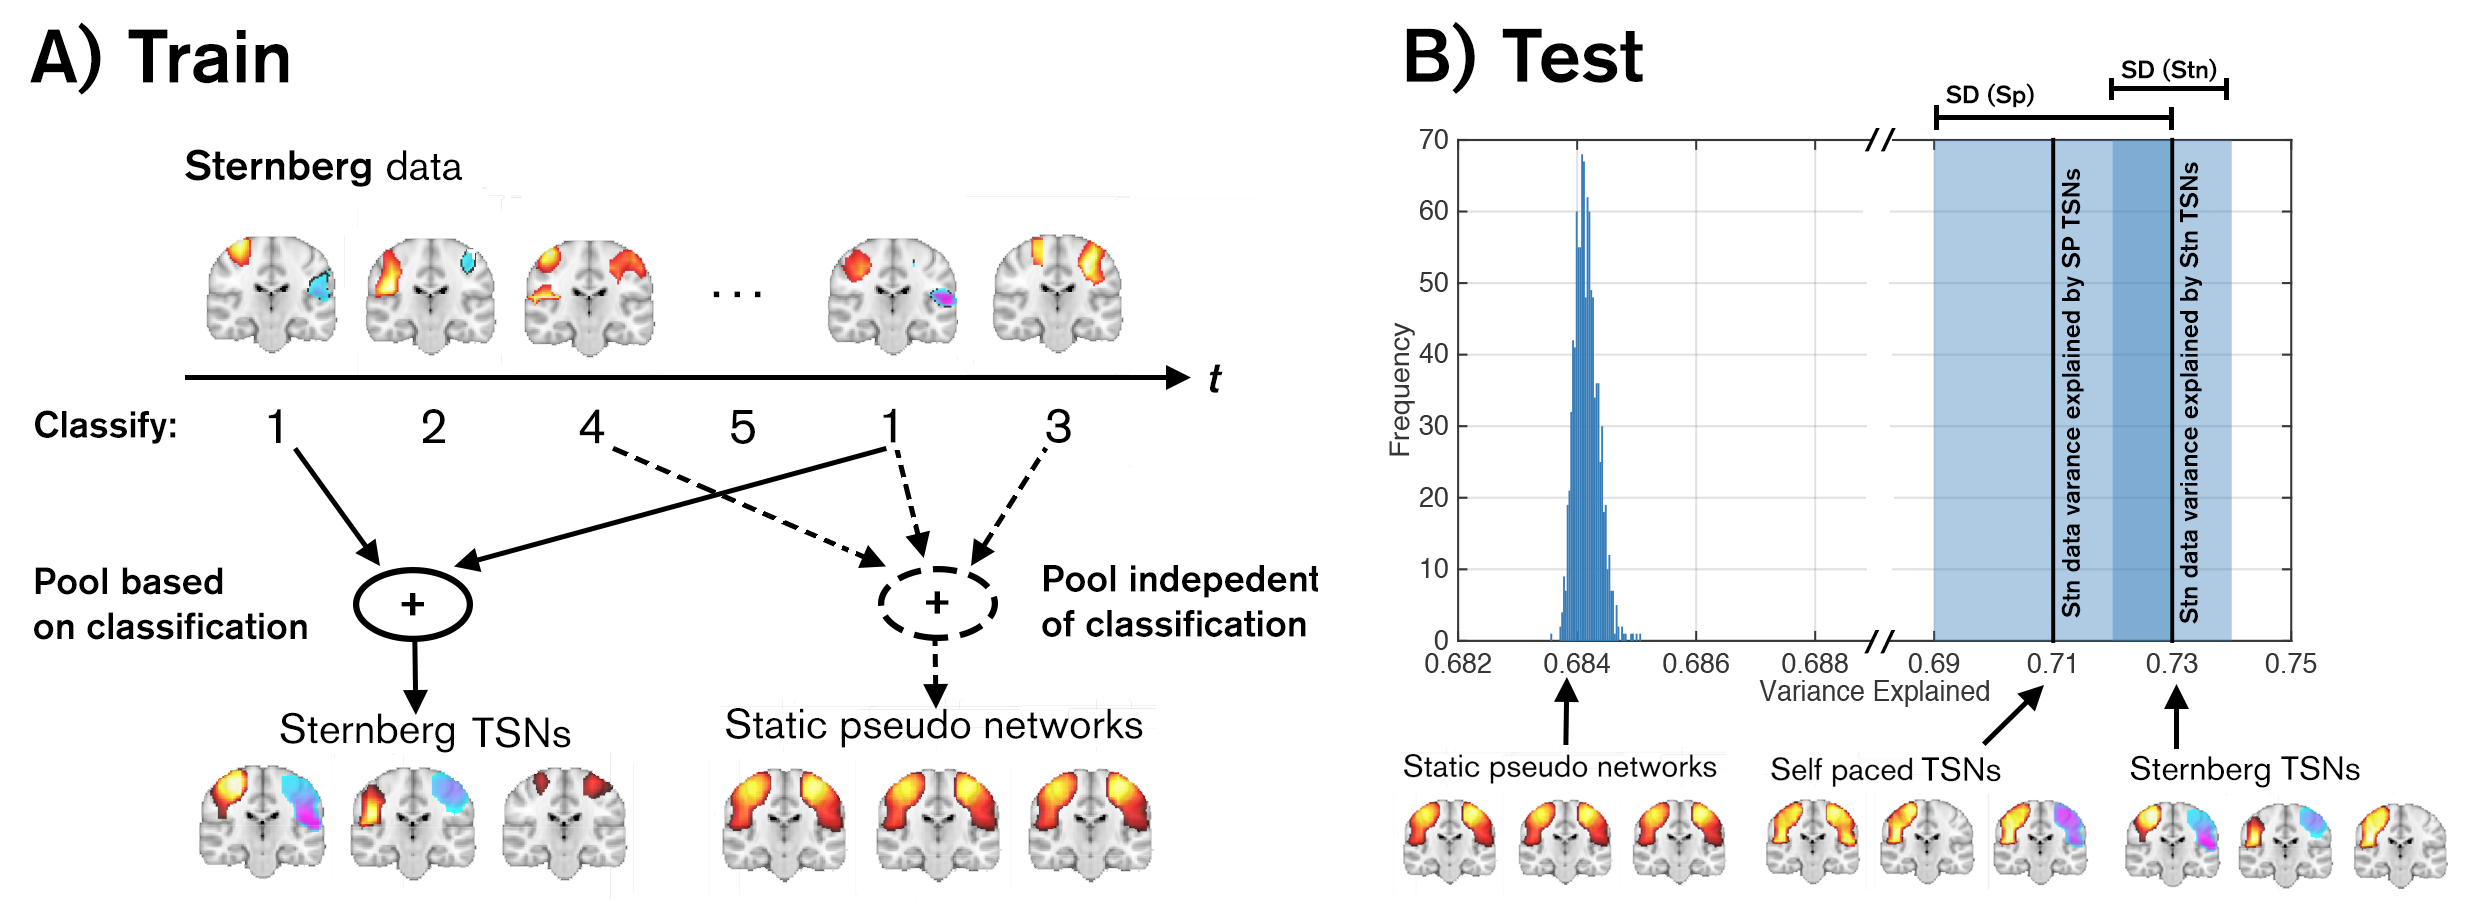
\includegraphics[width=\linewidth]{./images/chapter5/Figure_4.png}
		\caption{A) Schematic representation of the process to generate both the real TSNs, and a series of static pseudo-networks to test the null hypothesis. Real TSNs are generated based on the state allocation of individual connectivity images from the k-means clustering process, whislt for the pseudo static networks, states are assigned assuming stationarity. B) The resulting variance explained in the Sternberg connectivity data by 2000 permutations of the static pseudo networks (histogram) and the TSNs from both the self-paced and Sternberg datasets. Note that using self-paced rather than Sternberg TSNs to explain the Sternberg data does not result in a significant drop in variance explained, thus highlighting robustness of the TSN maps over experiments. Note also that the null hypothesis is rejected. \label{figure_5_4}}
	\end{center}
\end{figure*}
\end{landscape}

\subsection{Task induced change in functional connectivity}
Timecourses were generated to measure task induced changes in the probability of observing a specific TSN. An increase in these timecourses means that a TSN is more likely to be observed at a specific time point; a decrease means the TSN is less likely to be observed. Figure \ref{figure_5_5}A shows examples for self-paced data: timecourses represent the fractional change in probability for two selected TSNs. TSN6, which covers bilateral M1, exhibits a significant (\textit{p}<0.05) change around the time of the button press showing that we are ~200\% more likely to observe this TSN during a single finger movement (with one hand), compared to rest. Likewise TSN8, which covers bilateral sensory cortex also exhibits a significant (\textit{p}<0.05) task induced response. Similar results were observed for the Sternberg data and are shown in Figure \ref{figure_5_5}B. Here TSN7 (again bilateral M1) exhibits a significant (\textit{p}<0.05) change in occupancy around the time of the button press ($\bar{t}$= 8.41 s). The lower panel also shows probability timecourses, but contrasts trials with a fast reaction time (8.21\pm0.09 s), against trials with a slow reaction time (8.78 ± 0.59 s). Note the difference in time to peak and longevity of response. These results support the hypothesis that on task initiation the relative occupancy of TSN states is altered. 

\begin{figure*}[h]
	\begin{center}
		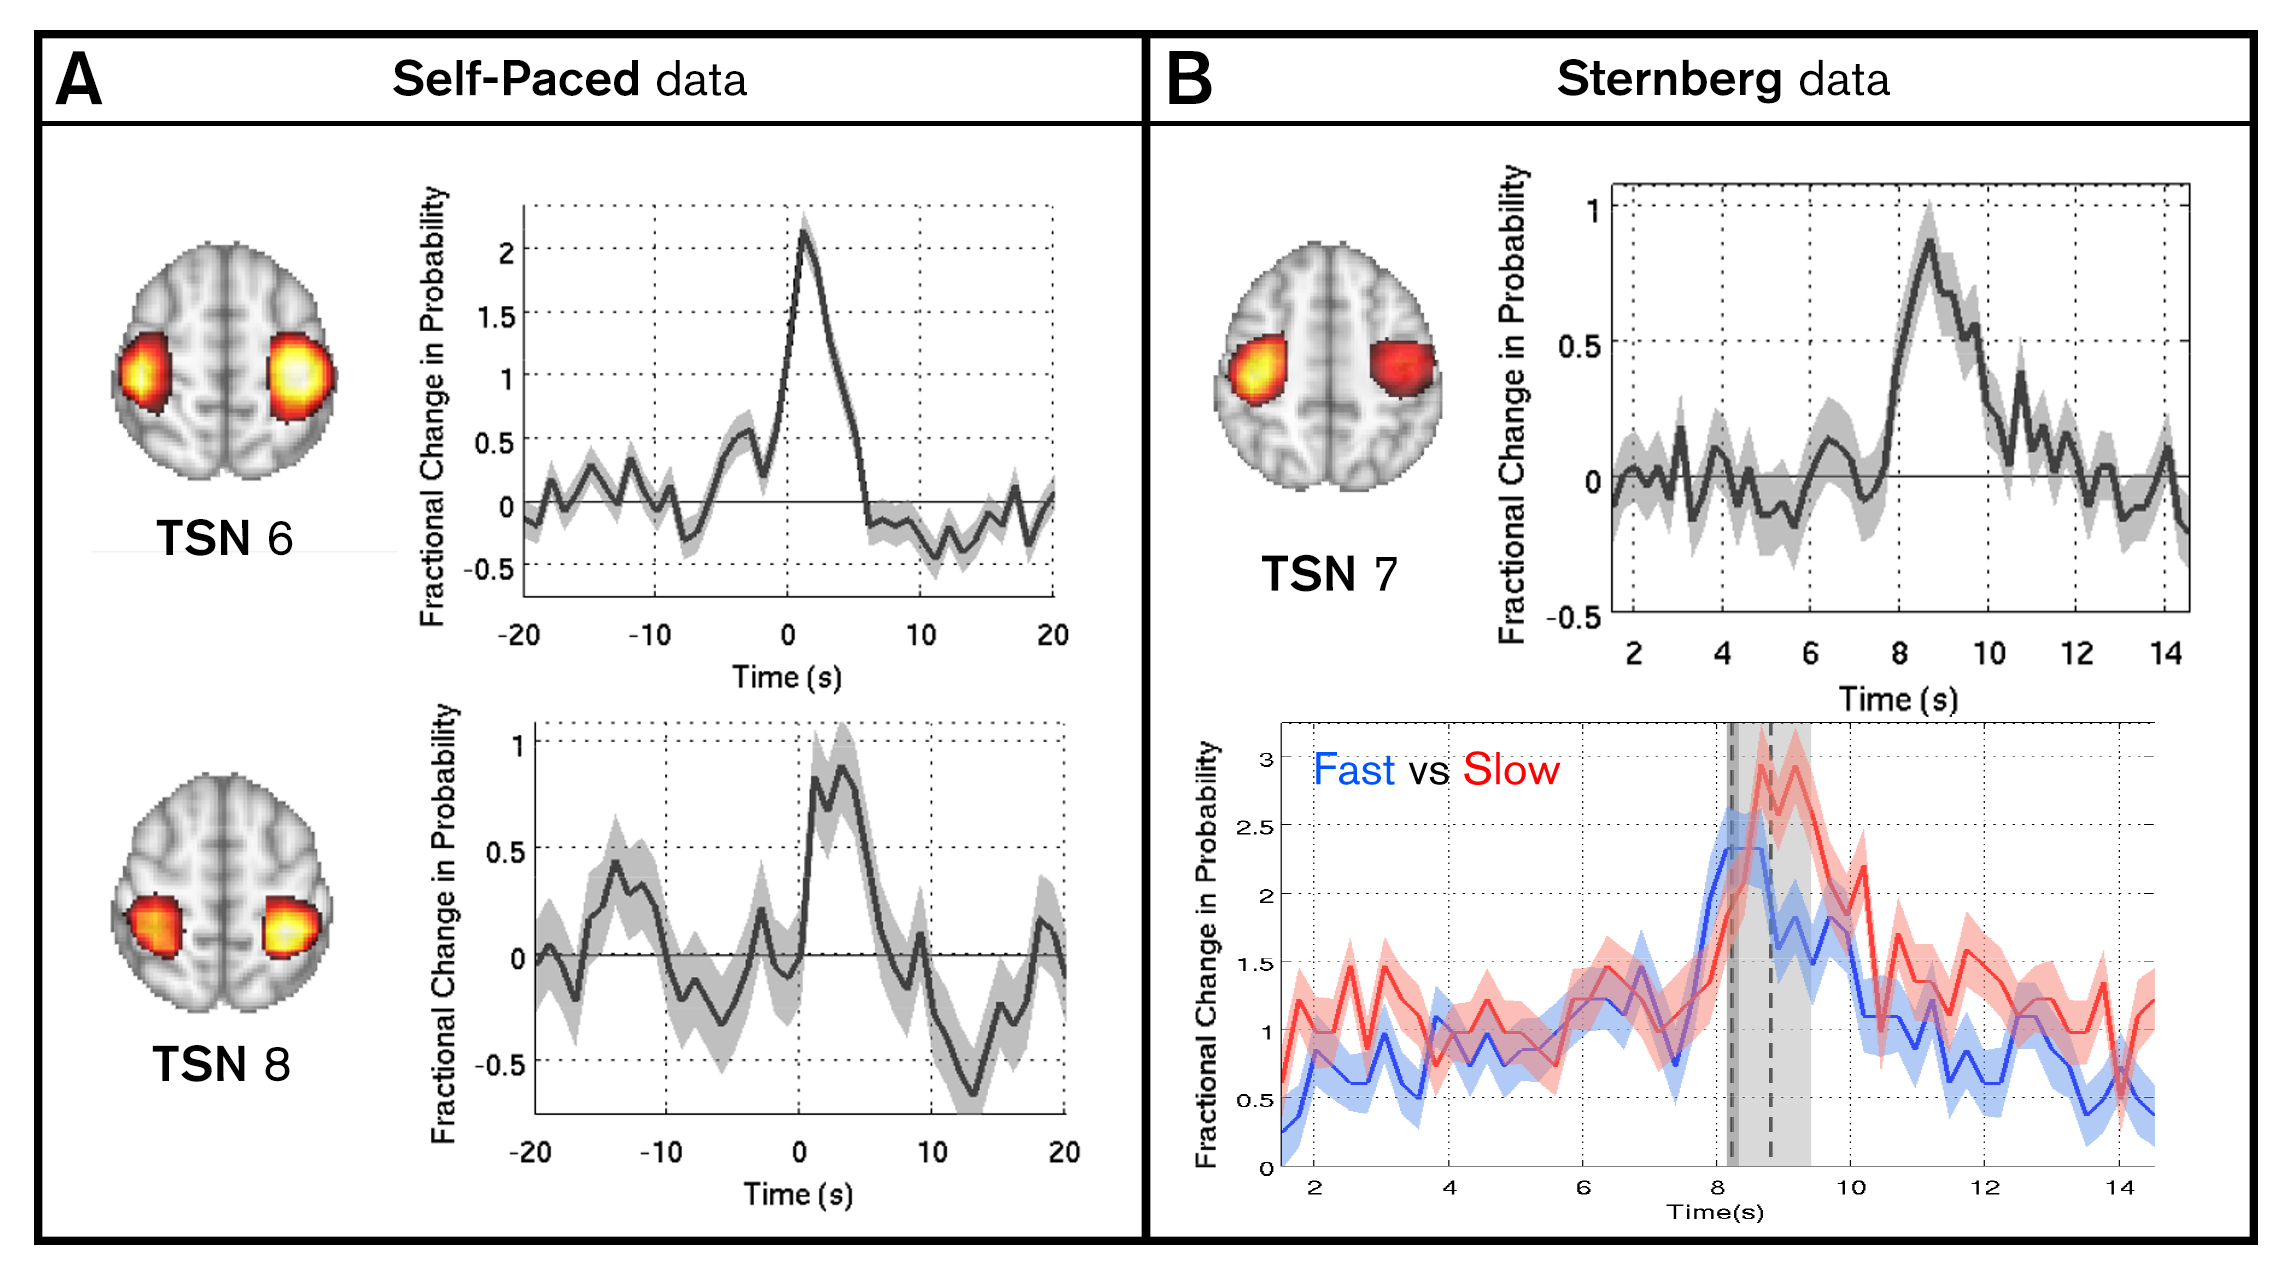
\includegraphics[width=\linewidth]{./images/chapter5/Figure_5.png}
		\caption{Task induced fractional change in TSN probability. A) shows the self-paced data. Note that only the two networks that exhibit a significant task induced change are shown. TSN6 covers bilateral motor cortex and TSN8 captures bilateral sensory cortex. B) shows the Sternberg data. The upper panel shows the trial average occupancy change for TSN7. The lower panel contrasts trials with a fast reaction time (8.21 ± 0.09 s, blue trace) with trials with a slow reaction time (8.78 ± 0.59 s, red trace). \label{figure_5_5}}
	\end{center}
\end{figure*}

Finally, Figure \ref{figure_5_6} probes the spatial and temporal scales of task induced change in functional connectivity. Figures \ref{figure_5_6}A and \ref{figure_5_6}B show trial averaged canonical correlation between clusters covering the sensorimotor network. The timecourses shown represent change in total inter-hemispheric functional connectivity within the sensorimotor system. Note that in both the self-paced and Sternberg experiments, a transient increase in connectivity between clusters is observable around the time of the button press. However, this increase is modest, as evidenced by the bar charts which show mean connectivity between clusters in windows capturing the button press compared to those capturing resting state. In the self-paced data, the variance explained in the test cluster by the seed was greater by 11±9\% in the windows containing the button press, whilst in the Sternberg data the same measure increased by 9±3\%; in both cases the change failed to reach statistical significance across subjects. Figures \ref{figure_5_6}C and \ref{figure_5_6}D show measured task induced change in functional connectivity between point locations selected on the basis of the TSN maps. Specifically, results show functional connectivity between primary motor areas (TSN6 for self-paced data and TSN7 in Sternberg data). Point-to-point connectivity is assessed using a univariate sliding window approach. Multiple window widths are shown collectively in the figure. Connectivity is averaged over task trials; the x-axis shows time relative to the button press, the y-axis shows log\textsubscript{10}(window width) and the colour shows connectivity strength (windowed correlation between beta envelope timecourses). The bar graphs show variance explained by the seed location at the test location. Windows encapsulating the button press are contrasted with those not encapsulating the button press.  Figures \ref{figure_5_5} and \ref{figure_5_6} are complementary. The increase in occupancy of specific TSNs during motor behaviour (Figure \ref{figure_5_5}) shows that efficient neural processing requires dominance of a specific sub-network to support movement. During movement, sensorimotor network functional connectivity is thus dominated by a small number of highly focal networks. This is evidenced by the increased functional connectivity between bilateral M1 in Figures \ref{figure_5_6}C and \ref{figure_5_6}D. However, this focal increase has relatively little effect on inter-hemispheric connectivity within the wider network (Figures \ref{figure_5_6}A and \ref{figure_5_6}B). 

\begin{landscape}
	\begin{figure*}
		\begin{center}
			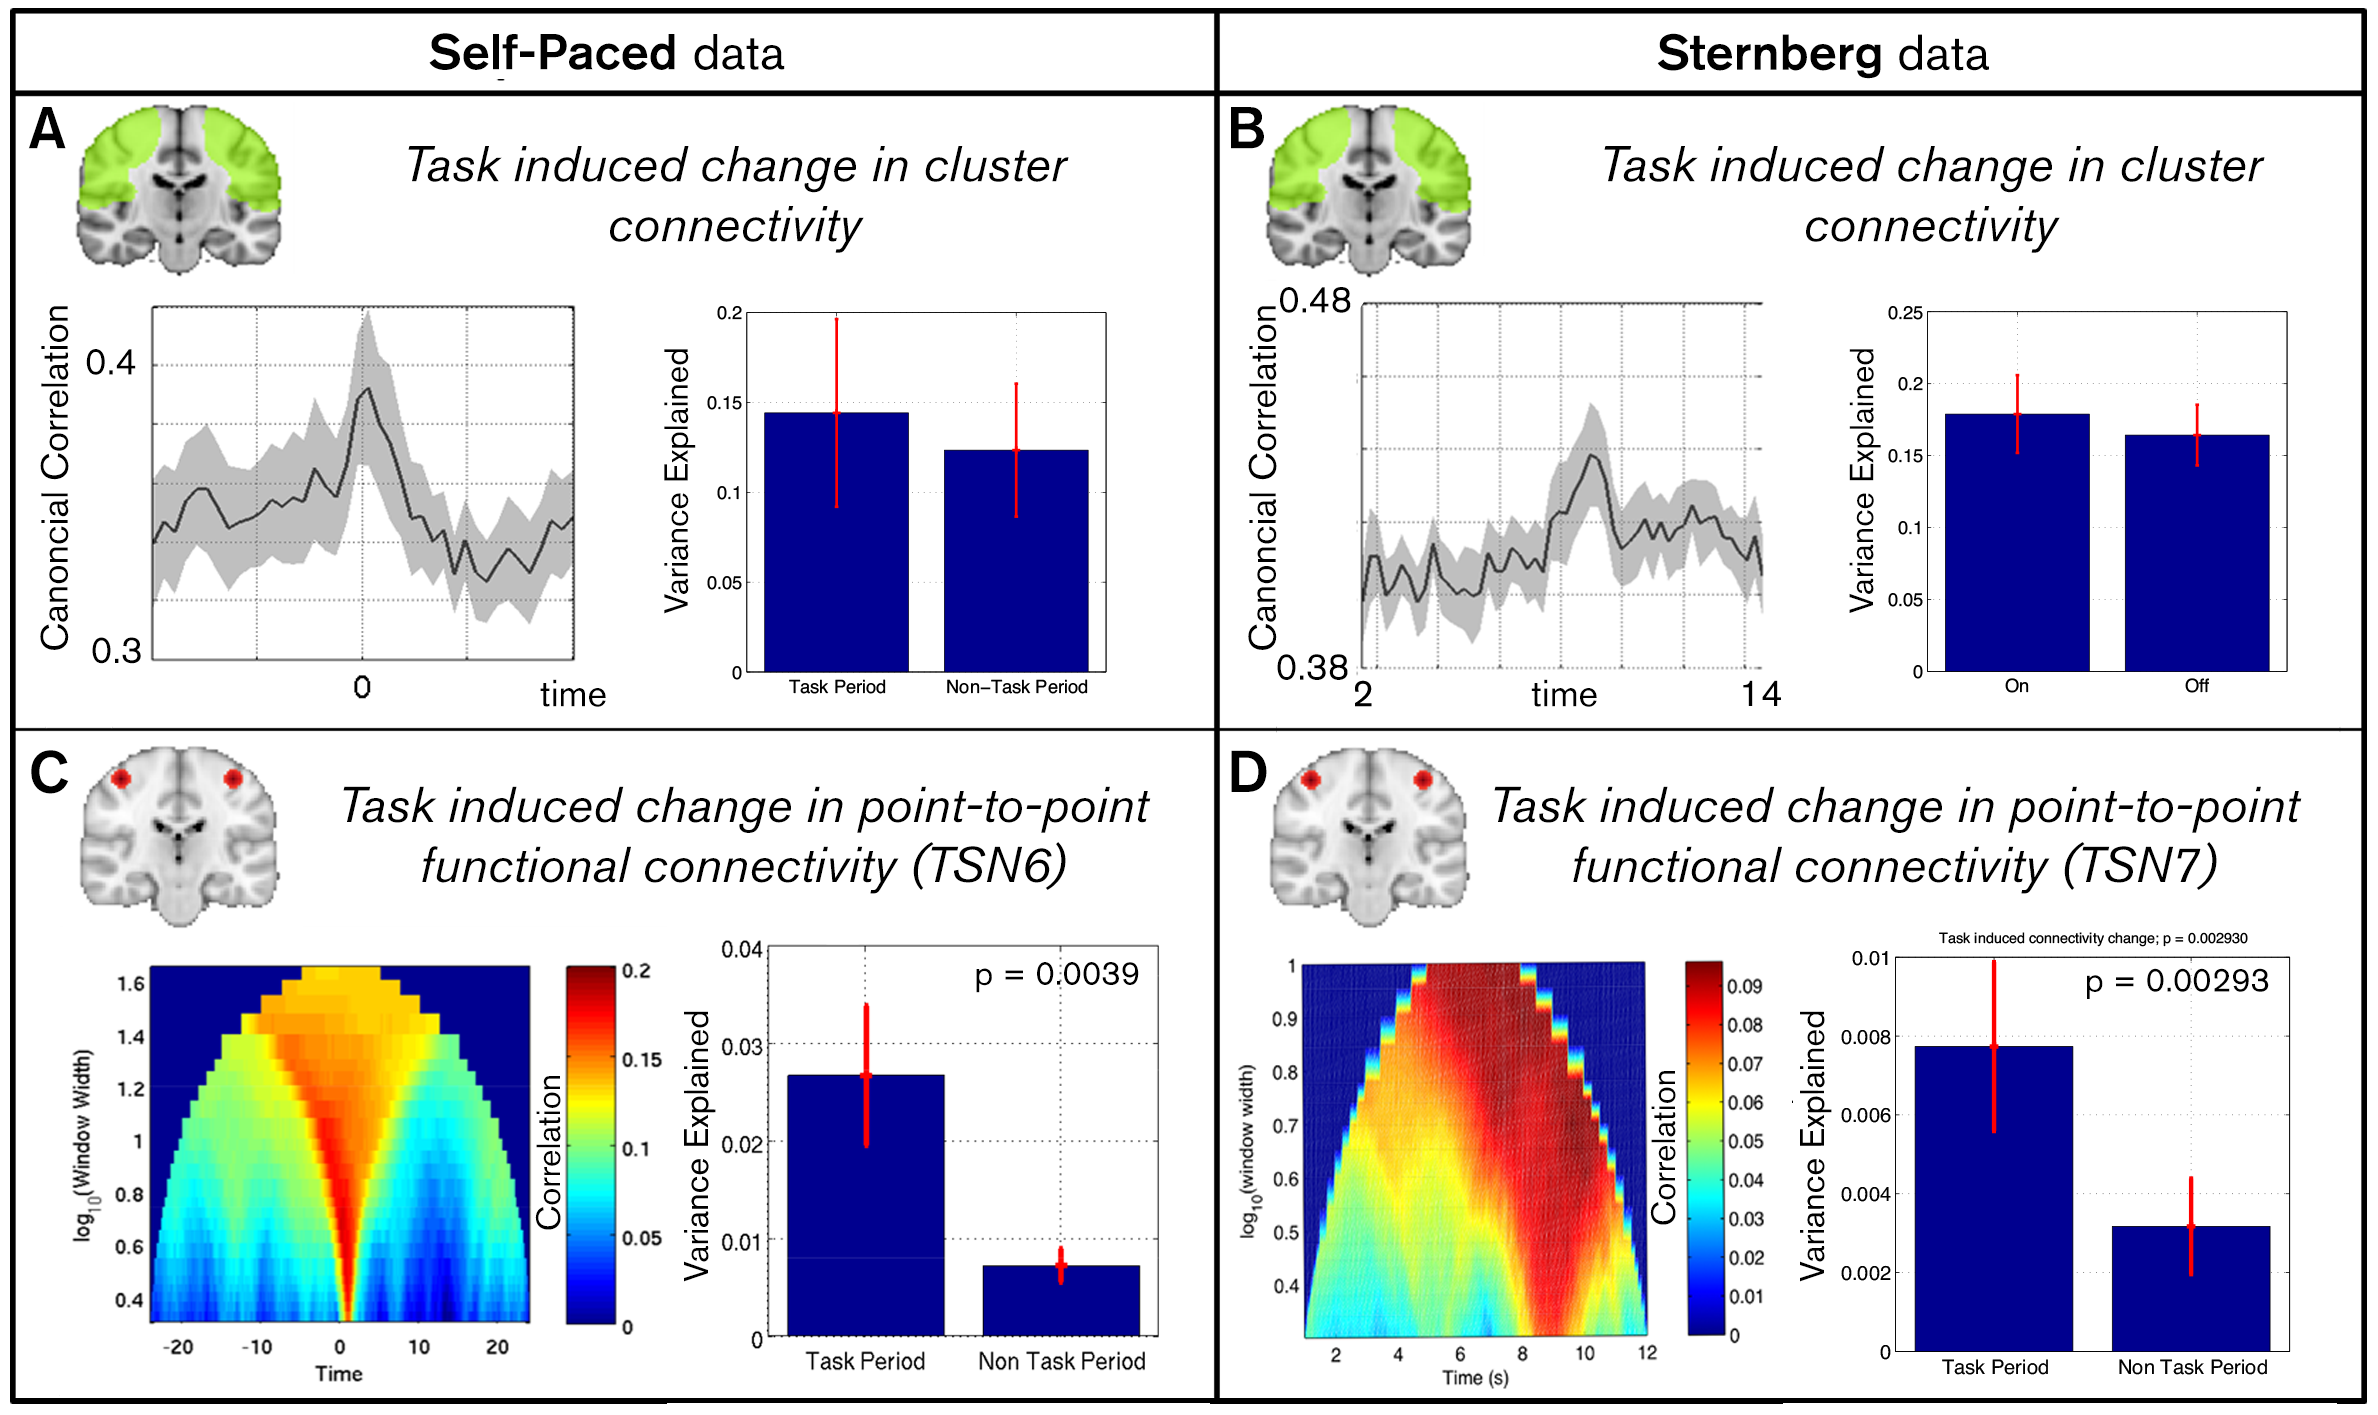
\includegraphics[width=0.8\linewidth]{./images/chapter5/Figure_6.png}
			\caption{Task induced change in functional connectivity at differing spatial and temporal scales. A/B) Connectivity between clusters. Timecourses show trial averaged response whereas bar charts show mean variance explained in the test cluster by the seed cluster, in windows capturing the button press compared to those not capturing the button press. C/D) Univariate connectivity between point locations. Pairs of voxels were selected based upon TSN6 (self-paced) and TSN7 (Sternberg). In the left hand plot the x-axis shows time relative to the button press, the y-axis shows log10(window width) and the colour shows the strength of connectivity (correlation between the Hilbert envelopes of beta oscillations, within the window). The bar graphs show variance explained by the seed location at the test location in windows encapsulating or not encapsulating the button press. \label{figure_5_6}}
		\end{center}
	\end{figure*}
\end{landscape}

\section{Discussion}\label{sec_kmeans_discus}
Using a new method for imaging transient patterns of functional connectivity, we have shown that the static metrics most often used to characterise coupling between network nodes fail to provide a complete picture of the complex spatio-temporal dynamics within the network they are attempting to describe. By exploiting the excellent time resolution of MEG, with advanced leakage reduction and multivariate connectivity modelling, we were able to show that the static sensorimotor network can be decomposed into multiple dynamically changing sub-networks. These sub-networks have been observed without the use of statistical priors and with unsurpassed spatiotemporal accuracy. We have shown that these TSNs are not only a common feature across subjects, but are also a common feature across completely independent multi-subject experiments. Indeed the evidence is that the commonly observed static network oversimplifies the ground truth: our data show clearly that individual areas of the larger network progress through stages of highly correlated, uncorrelated and even strongly anti-correlated activity. In addition we have shown that TSNs are a consistent feature of the resting state, and that task initiation serves to bias the likelihood of a particular TSN being recruited.

The observed spatial patterns represent physiologically interpretable networks of connectivity. Most noteworthy, our results show that, even outside a task, functionally specific and spatially focal brain areas can be extracted blindly. In some cases broad complexes of bilateral homologous regions were identified: For example in both studies the most commonly occurring TSN comprised bilateral M1 and S1, extending down to bilateral S2. Other networks revealed highly focal complexes, including bilateral primary motor area (M1), bilateral primary somatosensory area (S1) and bilateral secondary somatosensory area (S2), regions which resemble the modes of connectivity generated in Chapter \ref{chapter_cca} but this time over a group of subjects rather than one. In particular, the clear separation of motor (M1) and somatosensory (S1) cortices into two separate networks, despite these regions being separated by only a few millimetres, shows the spatial accuracy of the technique. The extraction of such neuroanatomical detail from MEG data is rare, particularly in the resting state. The existence of anti-correlated networks in both tasks suggests a transiently occurring antagonistic relationship between beta envelopes within some time windows. Such anti-correlation may result from random mind-wandering; for instance it is known that attending to a particular location in the body causes anti-correlated shifts in the amplitude of somatosensory beta band oscillations within the two hemispheres \citep{Bauer2012,VanEde2014}. Likewise imagining movement, or even specific body parts can cause similar effects \citep{Brinkman2014,DeLange2008}. The existence of an asymmetric network (covering right S2 and left S1/M1) is also interesting. It is known that transient connections between left M1/S1 and right S2 occur during tactile stimulus processing \citep{Simoes2003} and that connectivity between S1 and S2 has been associated with subjective perception \citep{Ploner2009}. This observation is therefore physiologically interpretable. 

An important point is that, although the results presented were obtained in the context of two disparate paradigms, neither were “pure resting state”. In our self-paced task, participants were pressing a button every 30 s but for the remainder of the period participants remained at rest. This allowed for confirmation of the existence of TSNs with the brain (apparently) at rest, and simultaneously enabled validation of our methodology for robustly uncovering task induced temporal fluctuations of sensorimotor sub-networks. This said, it is conceivable that differences may result between the resting phase of our self-paced task, and ‘pure’ resting state data (in which subjects lie in a scanner and “think of nothing”). To account for this limitation, our methodology was also applied to 10 minute “pure rest” recordings in 10 subjects (for results see Appendix \ref{sec_kmeans_app1}). Once again TSNs were largely similar with our methodology separating M1, S1 and S2 as well as identifying anti-correlated and as asymmetric networks. This, coupled with our statistical (“miss-a-TSN”) analyses shows convincingly that the TSNs presented are a consistent feature of the resting state sensorimotor system.

Our secondary hypothesis was that, on initiation of a motor task, efficient neural processing would favour recruitment of a specific set of transiently synchronising sub-networks. We have shown that functional connectivity between sub-network nodes in bilateral M1 consistently and transiently changes around the time of overt motor behaviour. This is evidenced by i) an increase in occupancy of the M1 TSN (Figure \ref{figure_5_5}) and ii) an increase in transient univariate connectivity measured between bilateral M1 (Figures \ref{figure_5_6}C and \ref{figure_5_6}D). Interestingly, these highly focal changes do not result in a drastic overall change in inter-hemispheric functional connectivity within the sensorimotor network (Figures \ref{figure_5_6}A and \ref{figure_5_6}B). At a practical level this is important: if region to region connectivity is measured the overall effect of a task may be ‘washed out’ across voxels. However, if point-to-point connectivity is assessed, this will likely result in significant task induced change. However, the latter necessarily relies on a-priori selection of the precise points to be considered; our TSN analysis, for the first time, offers a principled means to assess task induced changes in network connectivity without such confounds. At a more theoretical level this finding offers an interpretation of task induced connectivity. Figure \ref{figure_5_3} shows that sensorimotor network connectivity is maintained via several TSNs and, at rest, all of these spatial signatures, including those identified as relating to movement contribute to the high level of functional connectivity between the left and right sensorimotor strip. We speculate that active processing of a motor response simply involves the transient reorganisation of the resting state TSNs. This implies that active processing is not an additive process, but rests on simple spatial reorganisation of the wider sensorimotor network. Such a model explains the differences in connectivity across spatial scales shown in Figure \ref{figure_5_6} and should be further tested in future studies of task induced functional connectivity change using the same methodology.

\subsection{Technical Considerations}
The methodology that we introduce is critically dependent on the number of states to extract via k-means. \textit{k} must be selected prior to initiation and here, we chose $k=8$ which was set empirically. Whilst this potentially reflects a limitation, such empirical selection not uncommon and is analogous to methods employing ICA, in which number of components is often set by visual inspection of the output. Most importantly, using our ‘miss-a-TSN’ analysis, the contribution of each TSN to the overall explanation of variance in the connectivity images was assessed quantitatively. In this way, we were able to show whether removal of specific TSNs impacted significantly the variance explained in connectivity images. This analysis is key to avoid over fitting and should be undertaken by researchers using this technique.

Another crucial parameter is the width of the temporal window used to estimate functional connectivity. Here we used 6 s for the self paced motor data and 3 s for the Sternberg study. Our choice of window width made to ensure that different stimuli in each study were further apart than the window width and that their was enough effective data points in the window for CCA to correctly function (the lowest limit on window width, $\delta$ is $\sim \frac{2d}{B_w}$, where \textit{d} is the number of independent timecourses (determined by how many principal components were selected, which in this case was 4) and $B_w$ is the bandwidth of the data (17 Hz)). However for the self paced data, it can be seen that the full-width-half-maximum (FWHM) of the M1 subnetwork probability timecourse in Figure \ref{figure_5_5} is approximately the same as the window width. This implies that the window is not short enough as the underlying connectivity dynamics evolve on a shorter time scale (which is seen in Figure \ref{figure_5_6}). The question is how can we correctly assess what window is required? As mentioned above using CCA sets a lower bound but in general its worth following the principle suggested by \cite{Leonardi2015}, where on assessing the spectrogram of an envelope timecourse, the window width is determined as the inverse of the lowest peak frequency (unless the spectrum follows a 1/\textit{f} relation, meaning there is no optimal window size). 

As a final note, we should mention that in this chapter, following CCA we extract only the first eigenmode of connectivity to take forward to the subsequent k-means analysis. However, this reflects a potential limitation. For any single window there are up to $n_\text{voxels}-1$ further modes available that are (currently) ignored. These extra eigenmodes correspond to extra orthogonal mixtures of the features in the seed and test clusters that may also describe transient networks. It is possible (even likely) that the TSN maps shown in Figure \ref{figure_5_3} might also be represented in these higher order eigenmodes. For example, if a bilateral S2 network in window 1 becomes dominated by a bilateral S1 network in window 2, it is likely that the S2 network has not ‘disappeared,’ but rather persists at a lower level of functional connectivity and may well be represented by the extra eigenmodes. Harnessing these modes, and incorporating them into k-means clustering, would not only generate further insights and possibly allow tracking of individual transiently synchronising networks in time, but may also increase the effective number of averages contributing to the TSN maps, hence improve signal to noise. Future studies may wish to account for this.

\section{Conclusion} 
Resting state networks are of fundamental importance to neuroscience with evidence suggesting that they are integral to brain function and perturbed in pathology. However, the temporal dynamics of the functional connectivities underlying RSN structure are poorly understood. We have presented a framework to further our understanding of RSN dynamics. Using MEG, we have shown that the canonical sensorimotor network can be decomposed into transiently synchronising sub-networks, recruitment of which depends on current mental state. These sub-networks are highly focal, show rich temporal dynamics, and the interpretation is that the larger canonical network reflects only a temporal aggregate of transient functional sub-networks. The methodology developed opens new frontiers to study RSN dynamics; for example our technique could be applied to study other RSNs (e.g. DMN), between network connectivity, other frequency bands, different tasks, and patient populations. In this way, we have provided a new dimension in which to reveal the spatial, temporal and spectral signature of the human connectome.

\clearpage

\appsection
\section{APPEDNIX A: Temporal evolution of leakage}\label{sec_dyn_leak}

In this chapter we implemented leakage correction within each window rather than prior to a sliding window connectivity analysis. The reasons necessitating such measures are demonstrated in this Appendix, using an analytical model, simulations and analysis of real data.

\subsection{Charactersing Dynamic Leakage}
To demonstrate the requirement for dynamic leakage reduction in transient task based MEG connectivity analyses, it is worth revisiting the two source model introduced in Chapter \ref{chapter_fc_and_leakage}. Recalling Equation \ref{eqn_dyn_leak_0}, if we have two reconstructed sources $\hat{\mathbf{q}}_1$ and $\hat{\mathbf{q}}_2$, the modified estimated source timecourse ($\hat{\mathbf{q}}_{1M}$) following leakage reduction is:

\begin{equation}
\begin{aligned}
\hat{\mathbf{q}}_{1M} &= \hat{\mathbf{q}}_{1} - \beta\hat{\mathbf{q}}_{2}\\
&= (\mathbf{q}_{1} + a\mathbf{q}_{2})-\Bigg[\frac{a\sigma_2+b\sigma_1}{\sigma_2+b^2\sigma_1}\Bigg](\mathbf{q}_{2} + b\mathbf{q}_{1}).
\end{aligned}
\label{eqn_dyn_leak_1}
\end{equation} Where $a = \mathbf{w}^T_1\mathbf{l}_2$, $b = \mathbf{w}^T_2\mathbf{l}_1$ and $\sigma_x = \mathbf{q}_{x}\mathbf{q}_{x}^T$. Again, this simplfies to

\begin{equation}
\hat{\mathbf{q}}_{1M} = k(\sigma_2\mathbf{q}_1 - b\sigma_1\mathbf{q}_2),
\end{equation} where $k = \frac{1-ab}{\sigma_2+b^2\sigma_1}$ is a constant.  This model is now used to compute what happens in the case of the dynamic connectivity estimation. Assume first that the timecourse are broken in to windows; for simplicity we employ two contiguous windows, labelled $ a $ and $ b $, such that $\hat{\mathbf{q}}_{1M} = \begin{bmatrix}\hat{\mathbf{q}}_{1Ma}\\\hat{\mathbf{q}}_{1Mb}\end{bmatrix}$ and $\hat{\mathbf{q}}_{2} = \begin{bmatrix}\hat{\mathbf{q}}_{2a}\\\hat{\mathbf{q}}_{2b}\end{bmatrix}$. Considering the case where leakage reduction is applied based upon the whole timecourse, as per equation \ref{eqn_dyn_leak_1}, we estimate leakage within window $ a $. The leakage estimate for this single window can be computed as the correlation coefficient between $\hat{\mathbf{q}}_{1Ma}$ and $\hat{\mathbf{q}}_{2a}$, and should equal zero. Mathematicaly, the correlation coefficient is:

\begin{equation}
r = \frac{\hat{\mathbf{q}}_{1Ma}^T\hat{\mathbf{q}}_{2a}}{\sqrt{\hat{\mathbf{q}}_{1Ma}^T\hat{\mathbf{q}}_{1Ma}}\sqrt{\hat{\mathbf{q}}_{2a}^T\hat{\mathbf{q}}_{2a}}}.
\end{equation} Taking $\hat{\mathbf{q}}_{1Ma} = \hat{\mathbf{q}}_{1a} = \beta\hat{\mathbf{q}}_{2a} = k(\sigma_2\mathbf{q}_{1a} - \sigma_1\mathbf{q}_{2a})$, and assuming $\hat{\mathbf{q}}_{2a} = \mathbf{q}_{2a}+b\hat{\mathbf{q}}_{1a}$ (this further assumes that the beamformer covariance is computed over the whole experiment, so $b$ is invariant over time) then:

\begin{equation}
r = \frac{k}{\sqrt{\hat{\mathbf{q}}_{1Ma}^T\hat{\mathbf{q}}_{1Ma}}\sqrt{\hat{\mathbf{q}}_{2a}^T\hat{\mathbf{q}}_{2a}}}\big[(\sigma_2 \mathbf{q}_{1a}-\sigma_1b\mathbf{q}_{2a})^T(\mathbf{q}_{2a}+b\mathbf{q}_{2a})\big].
\end{equation} Assuming that the underlying source timecourses in window $a$ are orthogonal:

\begin{equation}
r = \frac{k}{\sqrt{\hat{\mathbf{q}}_{1Ma}^T\hat{\mathbf{q}}_{1Ma}}\sqrt{\hat{\mathbf{q}}_{2a}^T\hat{\mathbf{q}}_{2a}}}(\sigma_2b\mathbf{q}_{1a}^T\mathbf{q}_{1a}-\sigma_1b\mathbf{q}_{2a}^T\mathbf{q}_{2a})
\label{eqn_dyn_leak_2}
\end{equation} Returning to the definition of $\sigma_x = \mathbf{q}_x^T\mathbf{q}_x$ it can be seen that  $\sigma_x = N\nu_x^2$, where $ N $ is the number of samples in the timecourse and $\nu^2$ is the corresponding variance. Using this information to simplify Equation \ref{eqn_dyn_leak_2}, we arrive at

\begin{equation}
r = \frac{kN^2b(\nu^2_2\nu^2_{1a}-\nu^2_1\nu^2_{2a})}{{\sqrt{\hat{\mathbf{q}}_{1Ma}^T\hat{\mathbf{q}}_{1Ma}}\sqrt{\hat{\mathbf{q}}_{2a}^T\hat{\mathbf{q}}_{2a}}}}
\end{equation} If the variance of the test source is constant over all time, such that $\nu^2_{1a}=\nu^2_{1b}=\nu^2_{1}$ then $r\propto(\nu^2_2\nu^2_{1}-\nu^2_1\nu^2_{2a})$. We therefore see that only in the case where $\nu_{2a}^2=\nu_2^2$ will the windowed leakage estimate (post static leakage reduction) collapse to the required value of zero. In other words, in cases where the variance of the seed timecourse is invariant across separate windows, a static reduction adequately ensures zero leakage following leakage reduction. However, in cases where the seed variance changes between windows, the estimated leakage is non-zero and leakage reduction is required within each window of interest. Similar arguments can be put forward in the case of varying test signal variance across windows, or in cases where both the seed and test variance change across windows. 

\subsection{Methods}
In order to confirm the above analysis and asses the utility of dynamic leakage correction, a simulation and analysis of experimental data were undertaken. 

\subsubsection*{Simulation}
Six dipoles were simulated in locations of interest within the left and right sensorimotor strips. The first five dipoles comprised of 100 s of Gaussian distributed data (with a mean amplitude of 1.29 nAm). The sixth dipole was also Gaussian data but modulated temporally using 5 Hanning windows, each 20 s in duration. The standard deviation over all time of this source was 0.8 nAm. These simulated data were projected through a multiple spheres forward model and mixed with empty room noise. Source space reconstruction via beamforming to the simulated data and the magnitude of leakage was estimated between the left and right voxel clusters covering the left and right sensorimotor strips. Leakage reduction was achieved using the multivariate extension of the regression method which can be found in Chapter \ref{chapter_cca}. Note all six simulated timecourses are uncorrelated and so in the absence of leakage, we would expect to find zero correlation between the left and right clusters. Leakage was assessed in three cases: 1) with no leakage reduction 2) with static leakage reduction and 3) with dynamic leakage reduction applied.

\subsubsection*{Experimental Data}
In addition to the simulated case, we also estimated the effect of non-stationary leakage in real data. Leakage between the left and right sensorimotor strips was assessed in a single subject taking part in the a self-paced motor task, where the subject was asked to execute a button press with their index finger of their non dominant hand. The sensorimotor strips of the subject’s brain were isolated and masked. Source space data within these masks were reconstructed using the beamformer. Again leakage was reduced using the multi-variate method (Chapter \ref{chapter_cca}) on the reconstructed signals. Again, the magnitude of leakage was assessed under three conditions, with 1) no leakage reduction 2) static leakage reduction and 3) dynamic leakage reduction. The spatial profile of leakage across the left sensorimotor strip was also assessed.

\subsection{Results}
Figure \ref{figure_3_0}A shows results of the leakage reduction simulation. Figure \ref{figure_3_0}Ai shows the location of the six simulated sources along the left and right sensorimotor strips. Simulated timecourses for each source are also shown (inset) with 5 of the 6 sources having constant variance and the 6th having variance with temporal structure. The leakage profile was calculated between volumes of interest shown by the red overlay and covering the left and right sensorimotor regions. Leakage profile results (which were calculated as the average Pearson correlation between the seed timecourse and the test cluster), are shown in Figure \ref{figure_3_0}Aii: the red timecourse represents leakage with no reduction applied; the green timecourse shows leakage when a static reduction scheme is applied; the blue timecourse shows the case for dynamic leakage reduction. Note first that the leakage estimate contains significant temporal structure. This is most apparent in the case of no leakage reduction where the source timecourse shows clearly that the leakage profile tracks the variance of the modulating source in the seed cluster. It follows that without any leakage reduction applied, the result would not only be artefactually high functional connectivity estimates, but also artefactual functional connectivity estimates with temporal structure. When using static leakage reduction, the effect is reduced but nevertheless the leakage estimate is not driven to zero. When using the dynamic reduction scheme, the leakage estimate is zero, as required.

Figure \ref{figure_3_0}B shows dynamic leakage estimates in real MEG data. Figure \ref{figure_3_0}Bi shows the spatial profile of leakage from the left sensorimotor strip (the seed cluster), into the right sensorimotor strip (the test cluster). The coloured overlay shows the magnitude of the leakage across all voxels in the test cluster. The upper images show the case for a time window not capturing a button press. The lower image shows the case for a time window centred on a button press (in both cases no leakage reduction has been applied). Note that, in support of both the theoretical analyses and the simulation in Figure \ref{figure_3_0}A, temporal structure is observed in the leakage profile in real data. This observation is supported by Figure \ref{figure_3_0}Bii which shows the timecourse of leakage for a single voxel, averaged over all task trials in the self-paced button press paradigm. The red trace shows no leakage reduction whilst the black trace shows static leakage reduction.  It is important to note that, even with static leakage reduction, the change in variance of the beta band response, induced in the beamformer projected signal by the task, generates a change in the leakage profile. This in turn could be misinterpreted as a genuine task induced change in functional connectivity but is only a result of the imperfect reconstruction. It is however important to note that this effect is not observed in all subjects; this would be expected since the spatial resolution of the beamformer spatial filter (and therefore the spatial profile of signal leakage) will depend on a number of factors including overall signal to noise ratio of the data and source orientation. This inconsistency is highlighted in Figure \ref{figure_3_0}Biii, which shows the leakage timecourse for all voxels in the test cluster, plotted as a function of Euclidean distance from the centre of the seed cluster, for two subjects. Note that, for subject 1, leakage is task related with a clear increase around the button press (time zero). However, for subject five, no such effect is observed. 

\begin{figure}
	\begin{center}
		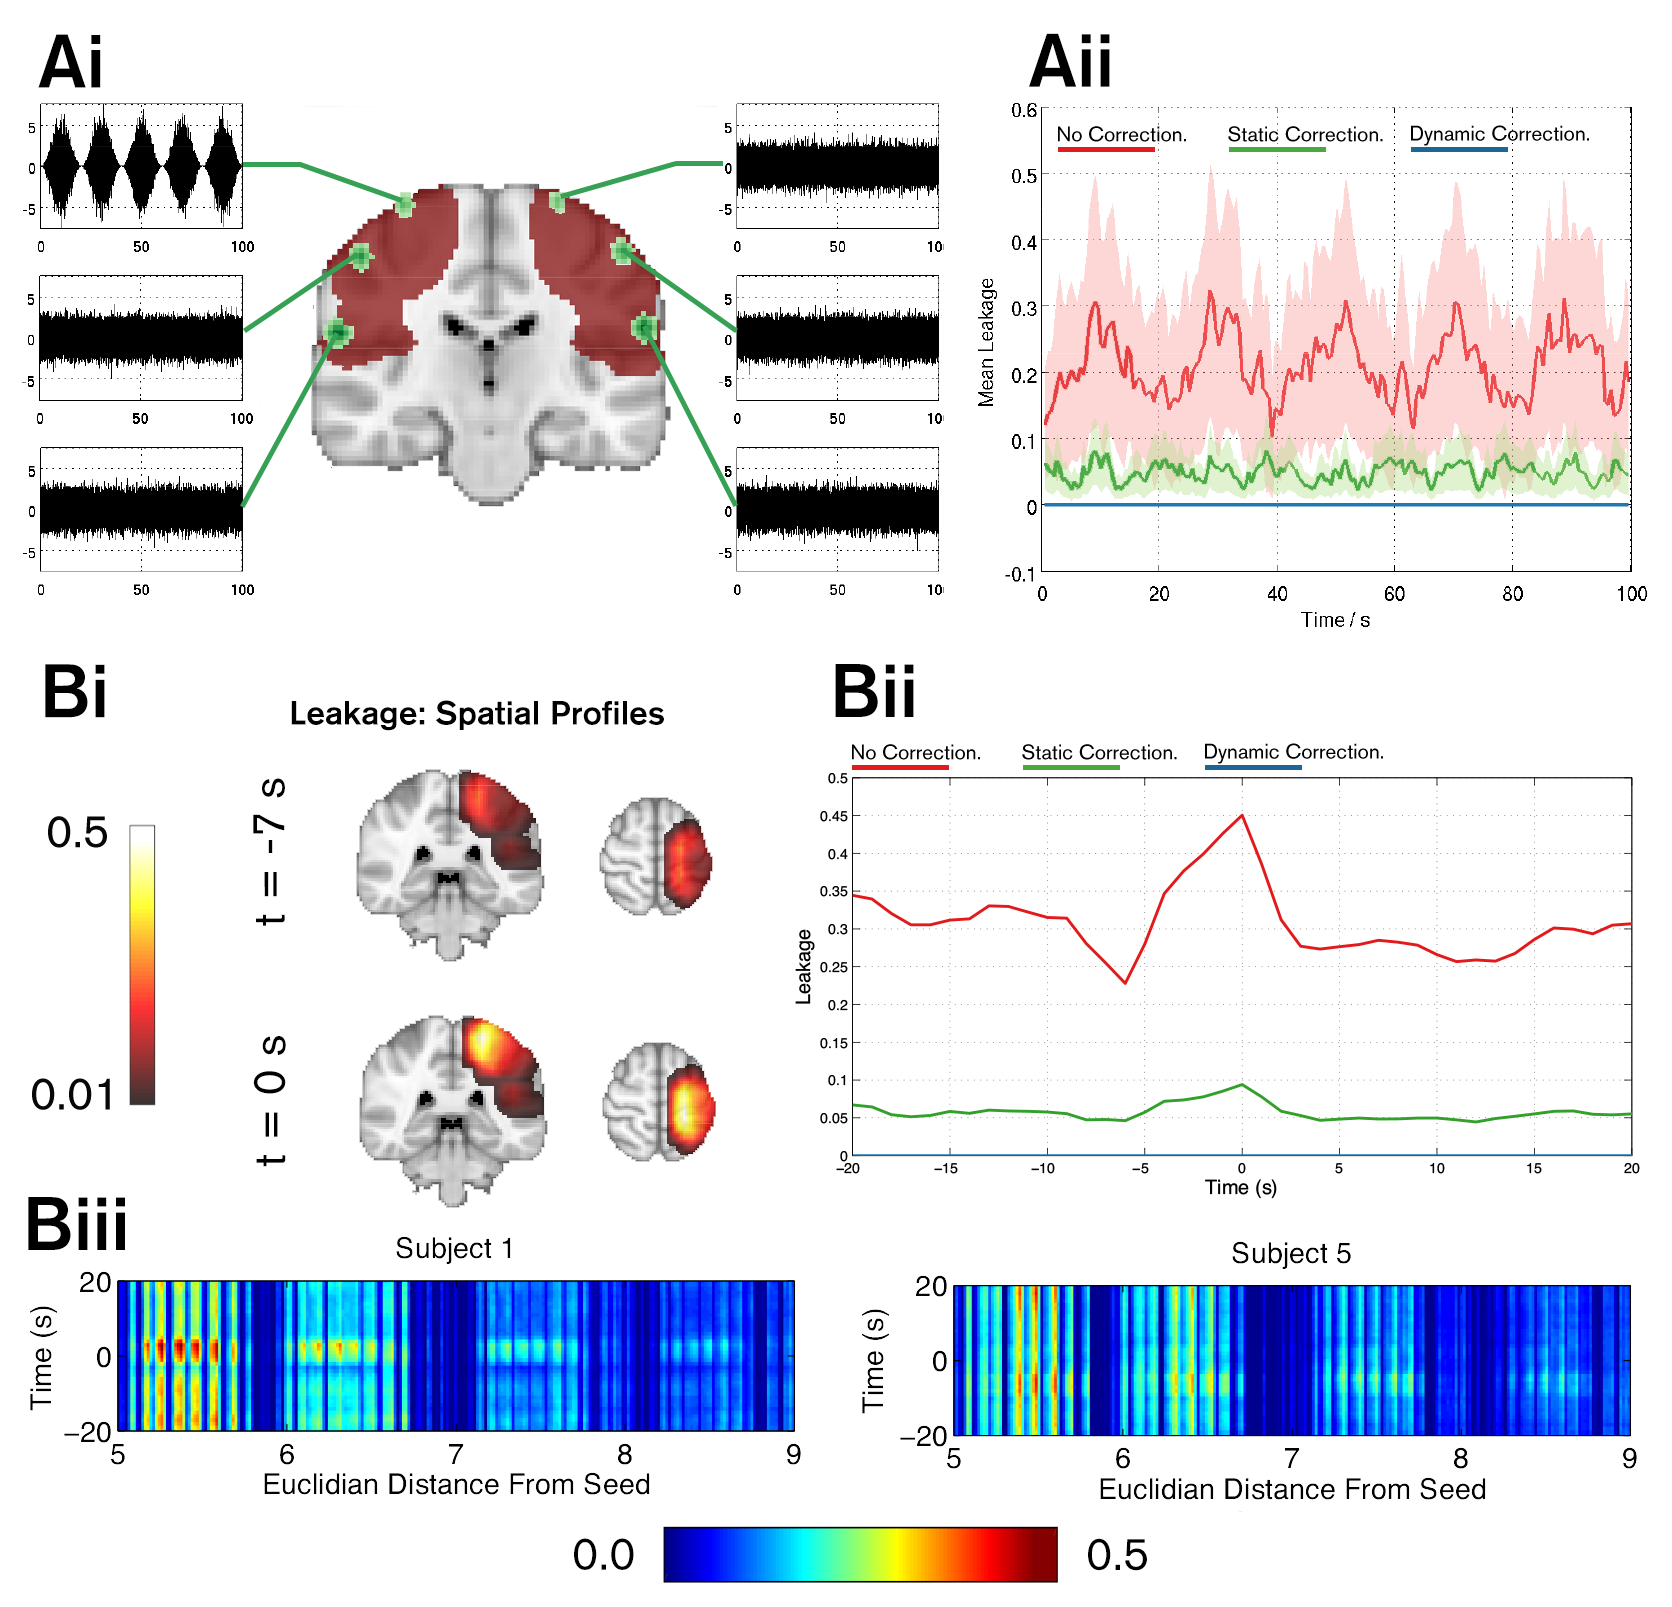
\includegraphics[width=0.95\linewidth]{./images/chapter3/Figure_0.png}
		\caption{The need for dynamic leakage reduction. A) Results of a 6 source simulation. Ai) The location of the 6 sources (green overlay) alongside the location of the seed and test clusters (red overlay) and the timecourses of each of the simulated sources (inset). Aii) Estimated source leakage from the seed (right sensorimotor strip) to the test (left sensorimotor strip) clusters. No leakage reduction (red), static leakage reduction (green) and dynamic leakage reduction (blue) are shown. B) Leakage in real data. Bi) the spatial profile of leakage for a window not containing a button press (upper panel) and a window containing a button press (lower panel). Bii) Timecourse of leakage estimate for a single voxel, averaged over trials, where 0s corresponds to the button press. Red shows no leakage reduction whilst black shows static leakage reduction – note increased leakage around the time of the event in both cases. Biii) Leakage timecourse for all voxels in the test cluster, for two subjects. Voxels, plotted down the x-axis, are ordered in terms of their Euclidean distance from the seed cluster. \label{figure_3_0}}
	\end{center}
\end{figure}

\clearpage

\section{APPENDIX B: TSN Generation from Pure Resting State Data}\label{sec_kmeans_app1}
In section \ref{sec_kmeans_discus}, we noted that “pure resting state” MEG data are typically recorded when a subject is asked to lie in a system and “think of nothing”. Distinct from this here, we employed a mixed approach, of interleaving a task with the resting state. This allowed us to both probe the existence of TSNs in the resting state, and validate our methodology with respect to its capability to elucidate temporal fluctuations of sub-network occupancies during the task. However, further validation to test for the presence of TSNs in pure resting state data would be of some value. With this in mind, we applied our technique to a separate multi-subject “pure” resting state dataset. 

Ten subjects took part in a ‘pure resting state’ study. Each subject was asked to lie in the MEG system with their eyes open and think of nothing whilst 600 s of resting state data were acquired using the protocols laid out in Chapter \ref{sec_data_acq}. Data analyses were the same as those used for the self-paced and Sternberg datasets. The spatial signatures of the 8 derived transiently synchronising sub-networks are shown in Figure \ref{figure_5_7}. Note the similarity between what is shown here and the equivalent maps shown in Figure \ref{figure_5_3}, and that M1 and S1 networks are separated.

\begin{figure*}[h]
	\begin{center}
		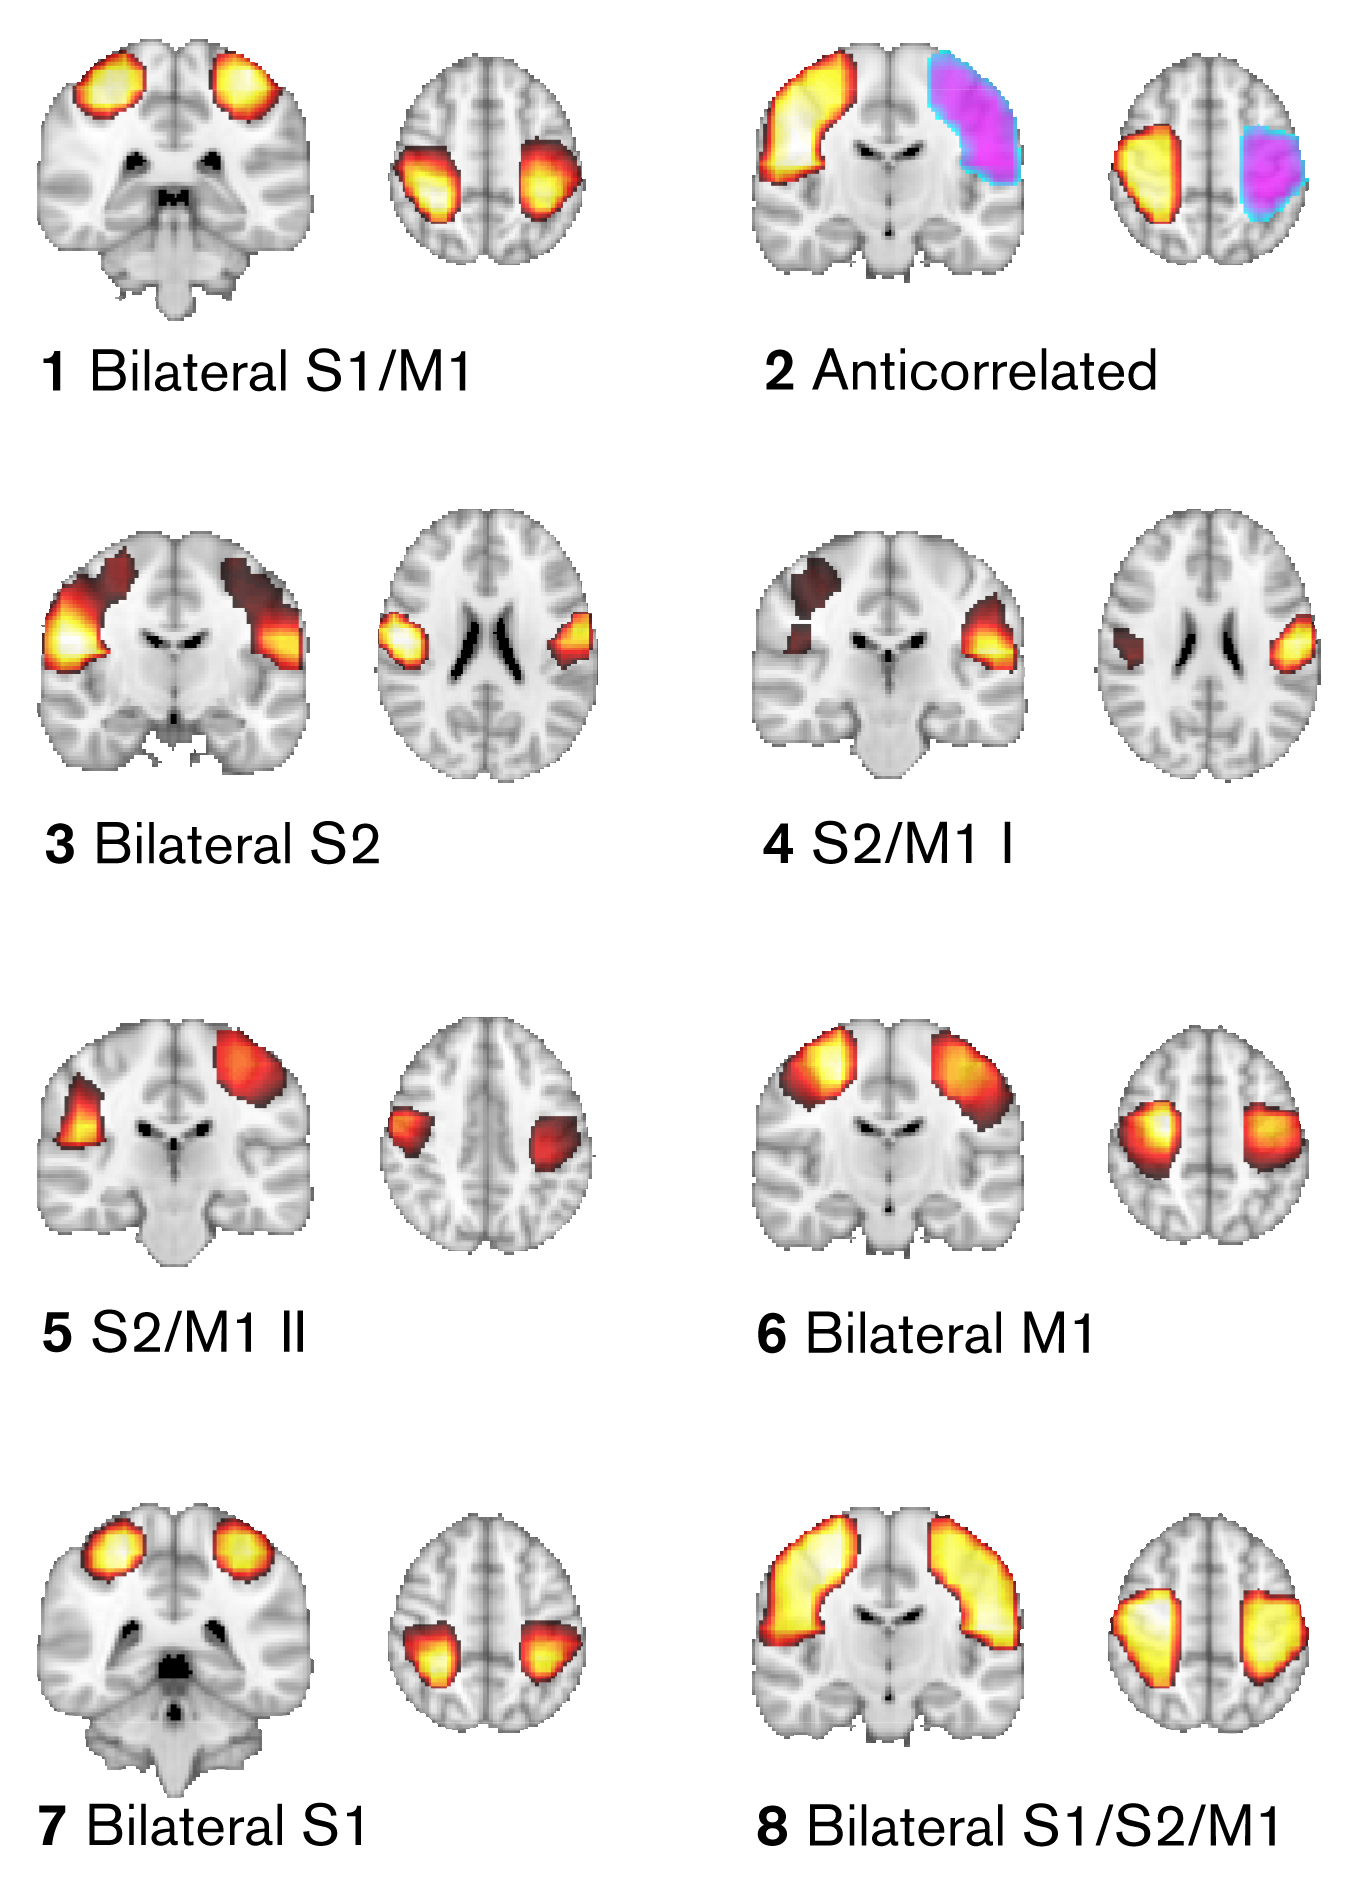
\includegraphics[width=0.75\linewidth]{./images/chapter5/Figure_7.png}
		\caption{TSN maps derived from pure resting state data in 10 subjects. Their topographies resemble those found in the self paced motor and Sternberg tasks, supporting the hypothesis that the TSNs are a fundamental process found in the resting state.\label{figure_5_7}}
	\end{center}
\end{figure*}